% Báo cáo đồ án CTDL & GT — biên dịch bằng XeLaTeX (build_report.ps1).
\documentclass[12pt,a4paper]{report}
\usepackage{fontspec}
\setmainfont{Times New Roman}
\setmonofont{Consolas}[Scale=MatchLowercase]

\usepackage[a4paper,margin=2.5cm]{geometry}
\usepackage{amsmath}
\usepackage{xcolor}
\usepackage{graphicx}
\usepackage{booktabs}
\usepackage{longtable}
\usepackage{tabularx}
\usepackage{array}
\usepackage{enumitem}
\usepackage{caption}
\usepackage{float}
\usepackage{fancyhdr}
\usepackage{titlesec}
\usepackage{listings}
\usepackage{algorithm}
\usepackage{algpseudocode}
\usepackage{tikz}
\usetikzlibrary{positioning,arrows.meta,fit,shapes.geometric,backgrounds}
\usepackage[unicode,hidelinks]{hyperref}

\linespread{1.15}
\emergencystretch=3em
\setlength{\parskip}{4pt}
\setlength{\parindent}{0pt}
\setlist{itemsep=2pt,topsep=3pt}

% Tên mục bằng tiếng Việt (không dùng babel/polyglossia để khỏi cần gói ngôn ngữ).
\renewcommand{\contentsname}{Mục lục}
\renewcommand{\listfigurename}{Danh mục hình}
\renewcommand{\listtablename}{Danh mục bảng}
\renewcommand{\figurename}{Hình}
\renewcommand{\tablename}{Bảng}
\renewcommand{\chaptername}{Chương}
\renewcommand{\bibname}{Tài liệu tham khảo}
\renewcommand{\appendixname}{Phụ lục}
\floatname{algorithm}{Thuật toán}
\renewcommand{\algorithmicrequire}{\textbf{Đầu vào:}}
\renewcommand{\algorithmicensure}{\textbf{Đầu ra:}}
\algrenewcommand\algorithmicif{\textbf{nếu}}
\algrenewcommand\algorithmicthen{\textbf{thì}}
\algrenewcommand\algorithmicelse{\textbf{ngược lại}}
\algrenewcommand\algorithmicfor{\textbf{với}}
\algrenewcommand\algorithmicdo{\textbf{thực hiện}}
\algrenewcommand\algorithmicwhile{\textbf{khi}}
\algrenewcommand\algorithmicreturn{\textbf{trả về}}
\algrenewcommand\algorithmicend{\textbf{kết thúc}}
\algrenewcommand\algorithmicloop{\textbf{lặp}}
\algrenewcommand\algorithmicrepeat{\textbf{lặp}}
\algrenewcommand\algorithmicuntil{\textbf{đến khi}}
\algrenewtext{EndIf}{\algorithmicend\ \algorithmicif}
\algrenewtext{EndFor}{\algorithmicend\ \algorithmicfor}
\algrenewtext{EndWhile}{\algorithmicend\ \algorithmicwhile}
\algrenewtext{EndProcedure}{\algorithmicend\ thủ tục}
\algrenewtext{Procedure}[2]{\textbf{thủ tục} \textsc{#1}(#2)}
\algrenewtext{Function}[2]{\textbf{hàm} \textsc{#1}(#2)}
\algrenewtext{EndFunction}{\algorithmicend\ hàm}

\titleformat{\chapter}[display]{\bfseries\Large}{\chaptername\ \thechapter}{8pt}{\LARGE}
\titlespacing*{\chapter}{0pt}{-10pt}{16pt}

\pagestyle{fancy}
\fancyhf{}
\fancyhead[L]{\small Quản lý mượn trả thiết bị Lab}
\fancyhead[R]{\small Lê Trường Khải — 25300003}
\fancyfoot[C]{\thepage}
\renewcommand{\headrulewidth}{0.4pt}
\fancypagestyle{plain}{\fancyhf{}\fancyfoot[C]{\thepage}\renewcommand{\headrulewidth}{0pt}}

\lstset{
  basicstyle=\ttfamily\small,
  breaklines=true,
  columns=fullflexible,
  keepspaces=true,
  frame=single,
  framerule=0.3pt,
  rulecolor=\color{black!30},
  backgroundcolor=\color{black!3},
  xleftmargin=4pt, xrightmargin=4pt,
  language=C++,
  keywordstyle=\bfseries,
  commentstyle=\itshape\color{black!60},
  showstringspaces=false
}

\newcommand{\code}[1]{\texttt{\detokenize{#1}}}
\newcommand{\bigO}[1]{$O(#1)$}

% Kiểu TikZ dùng chung cho các hình cấu trúc dữ liệu.
\tikzset{
  lnode/.style={draw,rounded corners=1pt,minimum height=0.8cm,minimum width=1.4cm,fill=white,font=\small\ttfamily},
  layer/.style={draw,rounded corners=3pt,minimum height=1.1cm,align=center,fill=black!4,font=\small},
  ptr/.style={-{Stealth[length=2mm]},thick},
  ptrback/.style={-{Stealth[length=2mm]},thick,color=blue!60!black},
  note/.style={font=\scriptsize\itshape,color=black!70}
}

\begin{document}
\pagenumbering{roman}
\begin{titlepage}
\centering
{\large \textbf{ĐẠI HỌC QUỐC GIA THÀNH PHỐ HỒ CHÍ MINH}\\[2pt]
\textbf{TRƯỜNG ĐẠI HỌC KHOA HỌC TỰ NHIÊN}\\[2pt]
(HCMUS)}\\[1.2cm]

{\large Môn học: \textbf{Thực hành Cấu trúc dữ liệu và Giải thuật}}\\[2.2cm]

{\Huge\bfseries BÁO CÁO ĐỒ ÁN}\\[0.8cm]
{\LARGE\bfseries Phần mềm quản lý mượn trả thiết bị\\[4pt]
và gợi ý đồ dùng thực hành}\\[0.6cm]
{\large (Đề số 3)}\\[2.5cm]

\begin{tabular}{rl}
\textbf{Giảng viên hướng dẫn:} & ThS. Trần Tuấn Kiệt\\[6pt]
\textbf{Sinh viên thực hiện:} & Lê Trường Khải\\[6pt]
\textbf{MSSV:} & 25300003\\
\end{tabular}

\vfill
{\large Thành phố Hồ Chí Minh, tháng 01 năm 2027}
\end{titlepage}

\tableofcontents
\listoffigures
\listoftables

\clearpage
\pagenumbering{arabic}
\chapter{Giới thiệu và phân tích yêu cầu}

\section{Bối cảnh và mục tiêu}
Các phòng Lab của trường cho sinh viên mượn thiết bị thực hành (kính thực tế ảo, tay cầm điều khiển, Arduino, máy hàn \ldots) và sách hiếm. Số lượng mỗi loại có hạn, nên cần theo dõi ai đang mượn gì, khi nào phải trả, ai đang chờ, và gợi ý những thiết bị thường được mượn cùng nhau.

Đồ án thực hiện \textbf{đề số 3}: một phần mềm quản lý mượn trả có hàng đợi đặt trước và gợi ý thông minh dựa trên lịch sử mượn. Mục tiêu chính của môn học là \textbf{tự cài đặt đúng cấu trúc dữ liệu} và giải thích được độ phức tạp, nên toàn bộ lõi nghiệp vụ dùng ba cấu trúc tự viết:
\begin{itemize}
  \item \textbf{Danh sách liên kết kép} (\code{DoublyLinkedList}) lưu danh mục thiết bị, phiếu mượn và các danh sách kề;
  \item \textbf{Hàng đợi} liên kết đơn (\code{LinkedQueue}) làm hàng đợi đặt trước và hàng thông báo;
  \item \textbf{Đồ thị vô hướng có trọng số} (\code{Graph}) cài bằng danh sách kề, lưu quan hệ mượn kèm.
\end{itemize}
Phần mềm có hai giao diện dùng chung một lõi: chương trình console \code{app.exe} và ứng dụng web \code{LabApp.exe} (máy chủ API và giao diện trình duyệt, chạy offline).

\section{Yêu cầu của đề}
Đề yêu cầu bốn nhóm chức năng:
\begin{enumerate}
  \item \textbf{Quản lý thiết bị và người mượn:} lưu mã, tên, số lượng, trạng thái (Sẵn sàng / Đang mượn / Bảo trì); lưu người mượn và ngày hẹn trả.
  \item \textbf{Hàng đợi đặt trước có thời hạn:} thiết bị hết số lượng thì người mượn tiếp theo vào hàng đợi; khi có thiết bị được trả, hệ thống báo cho người đầu hàng và người này có 24 giờ để đến nhận; quá 24 giờ thì bị đưa xuống cuối hàng và quyền chuyển cho người kế.
  \item \textbf{Gợi ý thiết bị đi kèm:} đồ thị có đỉnh là thiết bị, trọng số cạnh tăng 1 mỗi lần một sinh viên mượn cả hai cùng lúc; khi chọn thiết bị A hiện 3 thiết bị thường mượn kèm A nhiều nhất.
  \item \textbf{Giao diện} hiển thị rõ trạng thái thiết bị.
\end{enumerate}
Đề chia hai mức: \emph{cơ bản} (danh sách liên kết kép, mượn/trả, tính ngày quá hạn, giao diện trạng thái) và \emph{nâng cao} (hàng đợi tự loại người chờ quá 24 giờ, đồ thị gợi ý).

\section{Đối chiếu yêu cầu và chức năng}
\begin{table}[H]
\centering
\caption{Đối chiếu yêu cầu của đề với chức năng đã cài đặt}
\label{tab:mapping}
\small
\begin{tabularx}{\textwidth}{@{}l>{\raggedright\arraybackslash}p{3.6cm}>{\raggedright\arraybackslash}X>{\raggedright\arraybackslash}p{3.2cm}@{}}
\toprule
Mức & Yêu cầu & Cách thực hiện & Nơi thể hiện \\
\midrule
Cơ bản & Danh mục thiết bị bằng danh sách liên kết kép & \code{DoublyLinkedList<Device>} chèn có thứ tự theo mã (\code{insertSorted}) & Menu 1--5; màn Thiết bị \\
Cơ bản & Mượn/trả, ngày hẹn trả & \code{borrowDevices}, \code{returnRecord}; hạn trả $=$ giờ mượn $+$ số ngày $\times 24$ & Menu 6, 7; màn Mượn, Trả \\
Cơ bản & Tính ngày quá hạn & \code{overdueDays} làm tròn lên; phạt 36.000\,đ/ngày/thiết bị (\code{long long}) & Menu 11; màn Quá hạn \& Lịch sử \\
Cơ bản & Hiển thị trạng thái & Trạng thái suy ra từ số lượng (M1), thanh tỷ lệ \code{available/borrowed/onHold/maintenance} & Menu 1; màn Tổng quan, Thiết bị \\
Nâng cao & Hàng đợi đặt trước, giữ 24 giờ & \code{LinkedQueue<Reservation>} mỗi thiết bị; \code{serveQueue}, \code{claimReservation} & Menu 8; màn Hàng đợi \\
Nâng cao & Quá 24 giờ thì đẩy xuống cuối, chuyển quyền & \code{expireReservations}, \code{moveFrontToBack}, \code{missCount}, dây chuyền M15 & Menu 12 (tua giờ); thanh đồng hồ \\
Nâng cao & Gợi ý 3 thiết bị mượn kèm & \code{Graph::addCoBorrow}, \code{topNeighbors}, \code{suggestCompanions}, \code{suggestForBasket} & Menu 10; màn Mượn, Đồ thị \\
\bottomrule
\end{tabularx}
\end{table}

\section{Phạm vi và những gì không làm}
Đồ án làm một mình, không có đăng nhập, phân quyền hay mã hoá (ngoài đề). Giao diện web là phần nâng điểm; bản console đã đầy đủ chức năng và là bản nộp an toàn.

\chapter{Quy ước nghiệp vụ}

Đề bài không nói rõ một số điểm, nên trước khi cài đặt đã chốt các quy ước dưới đây. Mọi đoạn mã và kiểm thử đều theo đúng các quy ước này.

\section{Quy ước chung}
\begin{itemize}
  \item \textbf{Mượn cùng lúc} nghĩa là các thiết bị nằm trong \emph{cùng một phiếu mượn}. Phiếu có $k$ thiết bị thì cộng $+1$ cho mọi cặp trong $k$ thiết bị (tức $k(k-1)/2$ cạnh).
  \item \textbf{Quá 24 giờ chưa nhận:} đẩy xuống cuối hàng và tăng \code{missCount}; khi \code{missCount} đạt 2 thì loại hẳn khỏi hàng. Cách này thoả cả ``đẩy xuống cuối'' lẫn ``tự động loại bỏ'' của đề.
  \item \textbf{Đơn vị được giữ cho hàng đợi} không tính vào \code{available}. Bất biến luôn đúng:
  \[\code{available} + \code{borrowed} + \code{onHold} + \code{maintenance} = \code{total}.\]
  \item \textbf{Thời gian} dùng đồng hồ giả lập \code{Clock} (đơn vị giờ), có lệnh tua thời gian để trình bày được logic 24 giờ và quá hạn. Lõi không gọi \code{time()}.
  \item \textbf{Tiền phạt} 36.000 đồng mỗi ngày quá hạn, mỗi thiết bị tính riêng (phiếu 2 thiết bị trễ 3 ngày: $2\times 3\times 36.000 = 216.000$ đồng). Trễ chưa tròn ngày vẫn tính 1 ngày; lưu bằng \code{long long}, không dùng số thực.
  \item \textbf{Không xoá cứng} thiết bị còn phiếu mượn hoặc còn người trong hàng đợi; chỉ được chuyển sang Bảo trì.
\end{itemize}

\section{Các quy ước M1--M19}
\begin{longtable}{@{}l>{\raggedright\arraybackslash}p{13.8cm}@{}}
\caption{Quy ước nghiệp vụ M1--M19}\label{tab:conventions}\\
\toprule
Mã & Nội dung \\
\midrule
\endfirsthead
\toprule
Mã & Nội dung (tiếp) \\
\midrule
\endhead
\bottomrule
\endfoot
\multicolumn{2}{@{}l}{\textit{Thiết bị và trạng thái}}\\
M1 & Trạng thái suy ra từ số lượng: \code{maintenance == total} $\Rightarrow$ Bảo trì; \code{available > 0} $\Rightarrow$ Sẵn sàng; còn lại $\Rightarrow$ Đang mượn. \code{onHold} chỉ là con số, không phải trạng thái. \\
M2 & Bảo trì theo số đơn vị: \code{sendToMaintenance(id, qty)} chỉ lấy từ \code{available}; \code{finishMaintenance(id, qty)} trả về \code{available} rồi phục vụ hàng đợi. \\
M3 & Sửa \code{total} chỉ khi $\code{newTotal} \ge \code{borrowed}+\code{onHold}+\code{maintenance}$; tăng \code{total} thì phục vụ hàng đợi. \\
M4 & Xoá thiết bị (khi đủ điều kiện) xoá cả đỉnh và các cạnh trong đồ thị; phiếu lịch sử giữ nguyên mã, hiển thị ``đã xoá''. \\
M5 & Mã và tên không chứa dấu phẩy, dấu \code{|} hay xuống dòng (lõi kiểm tra) để CSV không cần ngoặc kép. \\
\midrule
\multicolumn{2}{@{}l}{\textit{Mượn / trả}}\\
M6 & Phiếu nguyên tử: phiếu nhiều thiết bị mà có món hết hàng thì thất bại cả phiếu, thông điệp liệt kê món hết; không cập nhật đồ thị. \\
M7 & Mỗi thiết bị tối đa 1 đơn vị trong một phiếu; không trùng mã trong phiếu. \\
M8 & Trả cả phiếu một lần, không trả từng món. \\
M9 & Số ngày mượn hợp lệ 1--30; không giới hạn số phiếu của một sinh viên. \\
M10 & Không có bảng sinh viên riêng; MSSV và họ tên nằm trong phiếu và trong hàng đợi. \\
\midrule
\multicolumn{2}{@{}l}{\textit{Hàng đợi}}\\
M11 & Giữ hàng nhiều người: mỗi đơn vị rảnh được giữ cho người \emph{chưa được giữ} đứng đầu tiếp theo; những người đang giữ luôn là một đoạn đầu của hàng. \\
M12 & Không cho đặt trước khi \code{available > 0} (phải mượn trực tiếp); một sinh viên không đứng hai lần trong cùng một hàng. \\
M13 & Nhận thiết bị (claim) tạo phiếu 1 thiết bị; số ngày nhập lúc nhận (mặc định 7, hợp lệ 1--30). Phiếu 1 món không cộng cạnh đồ thị. \\
M14 & Người bị đẩy xuống cuối mà hàng chỉ còn mình họ thì được giữ lại 24 giờ mới; lỡ lần thứ 2 thì bị loại, đơn vị trở về \code{available}. \\
M15 & Hết hạn dây chuyền: khi tua nhiều giờ, người kế nhận quyền giữ tính từ \code{holdUntil} cũ của người trước (không phải từ ``bây giờ''); lặp đến khi không còn ai hết hạn $\le$ giờ hiện tại. \\
M16 & Có thao tác huỷ đăng ký; nếu người huỷ đang giữ thì chuyển quyền cho người kế. \\
\midrule
\multicolumn{2}{@{}l}{\textit{Đồ thị và khác}}\\
M17 & Top 3: trọng số giảm dần, hoà thì mã tăng dần; ít hơn 3 láng giềng thì trả ít hơn. Top 3 bỏ qua thiết bị Bảo trì; thiết bị hết hàng vẫn gợi ý kèm cờ hết hàng. Gợi ý lúc lập phiếu (\code{suggestForBasket}) cộng trọng số của cùng một thiết bị qua các món trong giỏ, loại món đã có trong giỏ, tối đa 3, tính trên đồ thị \emph{trước khi} cộng phiếu đang tạo. \\
M18 & \code{Clock} đếm giờ kể từ 01/01/2026 00:00. Giờ hiện tại và bộ đếm mã phiếu lưu trong \code{meta.csv}. \\
M19 & Phiếu mở quá hạn hiển thị số ngày quá hạn và phạt tạm tính theo đồng hồ hiện tại; phạt chốt lúc trả. Hạn trả $=$ giờ mượn $+$ số ngày $\times 24$ giờ (không làm tròn tới cuối ngày); quá hạn khi giờ hiện tại $>$ hạn (đúng bằng hạn chưa quá hạn); số ngày quá hạn làm tròn lên. \\
\end{longtable}

\section{Giải thích một số lựa chọn}
\textbf{Vì sao dùng \code{missCount} thay vì chỉ ``đẩy xuống cuối''?} Nếu chỉ đẩy xuống cuối thì một người không bao giờ đến nhận sẽ quay vòng mãi và chiếm chỗ của người khác; nếu loại ngay lần đầu thì không có ``đẩy xuống cuối'' như đề nói. Cho phép lỡ một lần rồi loại ở lần thứ hai là cách dung hoà.

\textbf{Vì sao tách \code{onHold} khỏi \code{available}?} Đơn vị đang được giữ hộ một người thì người khác mượn trực tiếp không được lấy mất. Nếu để lẫn trong \code{available} thì phải tra hàng đợi mỗi lần mượn; tách riêng thì kiểm tra tồn kho chỉ là một phép so sánh $O(1)$, và bất biến tổng bốn số $= \code{total}$ giúp phát hiện lỗi sớm.

\chapter{Kiến trúc hệ thống}

\section{Ba tầng}
Hệ thống chia thành ba tầng (Hình~\ref{fig:arch}). Lõi là phần được chấm điểm; hai tầng còn lại chỉ là lớp chuyển đổi và giao diện.

\begin{figure}[H]
\centering
\begin{tikzpicture}[node distance=0.9cm and 1.2cm]
  \node[layer,minimum width=5.6cm] (web) {\textbf{Web UI}\\HTML + CSS + JavaScript\\\scriptsize thư mục \code{web/}};
  \node[layer,minimum width=5.6cm,right=1.4cm of web] (con) {\textbf{Console}\\C++: \code{main.cpp}, \code{UI.cpp}\\\scriptsize menu, bảng, màu ANSI};
  \node[layer,minimum width=5.6cm,below=1.3cm of web] (api) {\textbf{API server}\\C++ + cpp-httplib + nlohmann/json\\\scriptsize thư mục \code{server/}};
  \node[layer,minimum width=12.6cm,minimum height=1.5cm,below=1.3cm of api,xshift=3.5cm,fill=black!10] (core) {};
  \node[font=\small,align=center] at (core.center) {\textbf{Lõi (C++, cấu trúc dữ liệu tự cài)}\\\code{DoublyLinkedList}\quad\code{LinkedQueue}\quad\code{Graph}\quad\code{LabManager}\quad\code{Storage}};
  \node[layer,minimum width=5cm,below=1cm of core] (csv) {\code{data/*.csv}\\\scriptsize 4 tệp: devices, borrow\_records, reservations, meta};
  \draw[ptr,<->] (web) -- node[right,note]{HTTP + JSON} (api);
  \draw[ptr] (api.south) -- ++(0,-0.45) -| ([xshift=-2cm]core.north);
  \draw[ptr] (con.south) -- ++(0,-0.45) -| ([xshift=2cm]core.north);
  \draw[ptr,<->] (core.south) -- node[right,note]{đọc/ghi} (csv.north);
\end{tikzpicture}
\caption{Kiến trúc ba tầng}
\label{fig:arch}
\end{figure}

\begin{itemize}
  \item \textbf{Lõi} (\code{include/}, \code{src/}) tự cài \code{DoublyLinkedList}, \code{LinkedQueue}, \code{Graph}. Lõi \emph{không} dùng \code{std::list}, \code{std::queue}, \code{std::map}, \code{std::priority_queue}, \code{std::vector}, \code{std::sort}; chỉ dùng \code{std::string}, các luồng tệp và \code{std::function} (cho callback). Lõi không có \code{cout}/\code{cin} và không biết gì về HTTP hay JSON.
  \item \textbf{Console} (\code{app.exe}) gọi trực tiếp API công khai của \code{LabManager}.
  \item \textbf{API server} (\code{LabApp.exe}) dùng cpp-httplib và nlohmann/json (header-only) để đổi JSON $\leftrightarrow$ lời gọi lõi, đồng thời phục vụ tệp tĩnh trong \code{web/}. Tầng này được dùng STL thoải mái vì không chứa nghiệp vụ.
  \item \textbf{Web} chạy hoàn toàn offline (không CDN); không tự tính nghiệp vụ, mọi số liệu lấy từ API. Hợp đồng giữa web và server là \code{docs/api.md}.
\end{itemize}

\section{Lõi tách khỏi giao diện}
Hàm lõi nhận tham số và trả kết quả có cấu trúc, ví dụ \code{BorrowResult} gồm \code{ErrorCode} (\code{enum class}), thông điệp và danh sách món hết hàng. Danh sách trả ra dưới dạng cấu trúc tự cài hoặc qua \code{forEachDevice(callback)}. Sự kiện (``đến lượt SV X nhận thiết bị Y'', ``SV X lỡ hạn, bị đẩy xuống cuối'') được lõi đẩy vào \code{LinkedQueue<Notification>}; console và web tự lấy ra hiển thị. Nhờ vậy cùng một lõi phục vụ hai giao diện và cho ra số liệu giống hệt nhau.

\section{Lưu trữ CSV}
Dữ liệu lưu trong \code{data/} gồm \code{devices.csv}, \code{borrow_records.csv}, \code{reservations.csv}, \code{meta.csv}; đọc khi khởi động, ghi sau mỗi thao tác thay đổi (ghi ra tệp \code{.tmp} rồi đổi tên). Chỉ lưu \textbf{dữ liệu gốc}; những gì suy ra được thì tính lại khi nạp: \code{available}, \code{borrowed}, \code{onHold}, \code{timesBorrowed} và toàn bộ đồ thị mượn kèm (không có \code{graph.csv}). Cách dựng lại nằm ở mục~\ref{sec:load}.

\section{Công cụ và môi trường}
Windows 11, g++ (MinGW-w64) 13.2.0 với C++17, không dùng \code{make}; các tập lệnh PowerShell \code{build.ps1}, \code{build_server.ps1}, \code{build_test.ps1}. Bản phát hành biên dịch với \code{-O2 -DNDEBUG -static} nên chạy được trên máy không cài MinGW.

\chapter{Thiết kế các cấu trúc dữ liệu}

Ký hiệu độ phức tạp: $n$ = số thiết bị (độ dài danh sách), $m$ = số phiếu, $q$ = độ dài hàng đợi, $V$ = số đỉnh, $E$ = số cạnh, $d$ = bậc của đỉnh đang xét, $k$ = số phần tử cần lấy. Các bảng Big-O dưới đây chép từ chú thích trong mã nguồn (\code{include/*.h}).

\section{Danh sách liên kết kép \code{DoublyLinkedList<T>}}
\subsection{Cấu trúc}
Mỗi nút có dữ liệu và hai con trỏ \code{prev}, \code{next}; danh sách giữ \code{head_}, \code{tail_} và \code{size_} (Hình~\ref{fig:dll}).

\begin{figure}[H]
\centering
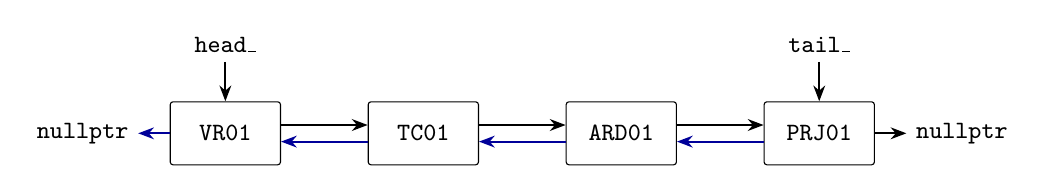
\begin{tikzpicture}[node distance=1.1cm]
  \node[lnode] (a) {VR01};
  \node[lnode,right=of a] (b) {TC01};
  \node[lnode,right=of b] (c) {ARD01};
  \node[lnode,right=of c] (d) {PRJ01};
  \draw[ptr] ([yshift=3pt]a.east) -- ([yshift=3pt]b.west);
  \draw[ptrback] ([yshift=-3pt]b.west) -- ([yshift=-3pt]a.east);
  \draw[ptr] ([yshift=3pt]b.east) -- ([yshift=3pt]c.west);
  \draw[ptrback] ([yshift=-3pt]c.west) -- ([yshift=-3pt]b.east);
  \draw[ptr] ([yshift=3pt]c.east) -- ([yshift=3pt]d.west);
  \draw[ptrback] ([yshift=-3pt]d.west) -- ([yshift=-3pt]c.east);
  \node[above=0.5cm of a,font=\small\ttfamily] (h) {head\_};
  \node[above=0.5cm of d,font=\small\ttfamily] (t) {tail\_};
  \draw[ptr] (h) -- (a);
  \draw[ptr] (t) -- (d);
  \node[left=0.4cm of a,font=\small\ttfamily] (n1) {nullptr};
  \node[right=0.4cm of d,font=\small\ttfamily] (n2) {nullptr};
  \draw[ptrback] (a.west) -- (n1);
  \draw[ptr] (d.east) -- (n2);
\end{tikzpicture}
\caption{Danh sách liên kết kép (mũi tên đen: \code{next}; mũi tên xanh: \code{prev})}
\label{fig:dll}
\end{figure}

\textbf{Dùng ở đâu:} danh mục thiết bị (\code{DoublyLinkedList<Device>}, sắp theo mã), danh sách phiếu mượn, danh sách mã thiết bị trong một phiếu, danh sách đỉnh và danh sách kề của đồ thị, và các danh sách kết quả gợi ý. Chọn danh sách kép vì \emph{gỡ một nút khi đã có con trỏ tới nó là $O(1)$} (nút biết \code{prev}) và có thể thêm/xoá ở cả hai đầu $O(1)$.

\subsection{Mã giả}
Hai thao tác lõi là chèn trước một nút và gỡ một nút; mọi thao tác khác (\code{pushFront}, \code{pushBack}, \code{insertSorted}, \code{erase}) dựa trên chúng.

\begin{algorithm}[H]
\caption{\textsc{LinkBefore}$(pos, value)$: chèn trước nút $pos$ ($pos=\text{null}$: chèn cuối)}
\begin{algorithmic}[1]
\State $n \gets$ nút mới chứa $value$
\If{$pos = \text{null}$}
  \State $n.prev \gets tail$
  \If{$tail \ne \text{null}$} \State $tail.next \gets n$ \Else \State $head \gets n$ \EndIf
  \State $tail \gets n$
\Else
  \State $n.next \gets pos$;\quad $n.prev \gets pos.prev$
  \If{$pos.prev \ne \text{null}$} \State $pos.prev.next \gets n$ \Else \State $head \gets n$ \EndIf
  \State $pos.prev \gets n$
\EndIf
\State $size \gets size + 1$
\end{algorithmic}
\end{algorithm}

\begin{algorithm}[H]
\caption{\textsc{Unlink}$(n)$: gỡ và giải phóng nút $n$}
\begin{algorithmic}[1]
\If{$n.prev \ne \text{null}$} \State $n.prev.next \gets n.next$ \Else \State $head \gets n.next$ \EndIf
\If{$n.next \ne \text{null}$} \State $n.next.prev \gets n.prev$ \Else \State $tail \gets n.prev$ \EndIf
\State giải phóng $n$;\quad $size \gets size - 1$
\end{algorithmic}
\end{algorithm}

\begin{algorithm}[H]
\caption{\textsc{InsertSorted}$(value, less)$: chèn giữ thứ tự tăng, ổn định}
\begin{algorithmic}[1]
\State $p \gets head$
\While{$p \ne \text{null}$ \textbf{và không} $less(value, p.data)$}
  \State $p \gets p.next$
\EndWhile
\State \Call{LinkBefore}{$p, value$}
\end{algorithmic}
\end{algorithm}

\subsection{Độ phức tạp}
\begin{table}[H]
\centering
\caption{Big-O của \code{DoublyLinkedList}}
\label{tab:dll}
\small
\begin{tabular}{@{}>{\raggedright\arraybackslash}p{6.0cm}>{\raggedright\arraybackslash}p{4.3cm}>{\raggedright\arraybackslash}p{4.7cm}@{}}
\toprule
Thao tác & Độ phức tạp & Ghi chú \\
\midrule
\code{pushFront}, \code{pushBack}, \code{popFront}, \code{popBack} & \bigO{1} & có cả \code{head_} lẫn \code{tail_} \\
\code{erase(it)} (gỡ nút đã có iterator) & \bigO{1} & nút biết \code{prev} \\
\code{insertSorted} & \bigO{n} & tìm vị trí, chèn \bigO{1} \\
\code{findFirst}, \code{removeFirst(pred)} & \bigO{n} & tìm \bigO{n} $+$ gỡ \bigO{1} \\
\code{forEach}, \code{removeAll(pred)}, \code{clear} & \bigO{n} & \\
\code{size}, \code{empty}, \code{swap}, di chuyển & \bigO{1} & \\
Sao chép sâu, gán (copy-and-swap) & \bigO{n} & an toàn khi tự gán \\
\code{checkIntegrity} & \bigO{n} & duyệt xuôi rồi ngược, kiểm \code{prev}/\code{next}, \code{size_} \\
\bottomrule
\end{tabular}
\end{table}

\section{Hàng đợi \code{LinkedQueue<T>}}
\subsection{Cấu trúc}
Hàng đợi chỉ đi một chiều từ đầu đến cuối nên dùng danh sách liên kết \emph{đơn} với hai con trỏ \code{head_} (người được phục vụ trước) và \code{tail_} (Hình~\ref{fig:queue}).

\begin{figure}[H]
\centering
\begin{tikzpicture}[node distance=1.1cm]
  \node[lnode] (a) {Khôi \#1};
  \node[lnode,right=of a] (b) {Nhi \#2};
  \node[lnode,right=of b] (c) {Bảo \#3};
  \draw[ptr] (a) -- (b);
  \draw[ptr] (b) -- (c);
  \node[above=0.5cm of a,font=\small\ttfamily] (h) {head\_};
  \node[above=0.5cm of c,font=\small\ttfamily] (t) {tail\_};
  \draw[ptr] (h) -- (a);
  \draw[ptr] (t) -- (c);
  \node[right=0.4cm of c,font=\small\ttfamily] (nn) {nullptr};
  \draw[ptr] (c) -- (nn);
  % sau moveFrontToBack
  \node[lnode,below=1.9cm of a] (a2) {Nhi \#1};
  \node[lnode,right=of a2] (b2) {Bảo \#2};
  \node[lnode,right=of b2] (c2) {Khôi \#3};
  \draw[ptr] (a2) -- (b2);
  \draw[ptr] (b2) -- (c2);
  \node[left=0.3cm of a2,font=\scriptsize\itshape,align=right] {sau\\\code{moveFrontToBack}};
  \node[right=0.4cm of c2,font=\small\ttfamily] (nn2) {nullptr};
  \draw[ptr] (c2) -- (nn2);
  \node[below=0.5cm of a2,font=\small\ttfamily] (h2) {head\_};
  \node[below=0.5cm of c2,font=\small\ttfamily] (t2) {tail\_};
  \draw[ptr] (h2) -- (a2);
  \draw[ptr] (t2) -- (c2);
\end{tikzpicture}
\caption{Hàng đợi liên kết đơn trước và sau \code{moveFrontToBack}: chỉ nối lại con trỏ, không cấp phát hay giải phóng}
\label{fig:queue}
\end{figure}

\textbf{Dùng ở đâu:} hàng đợi đặt trước của từng thiết bị (\code{LinkedQueue<Reservation>}) và hàng thông báo của lõi (\code{LinkedQueue<Notification>}).

\subsection{Mã giả}
\begin{algorithm}[H]
\caption{Các thao tác chính của \code{LinkedQueue}}
\begin{algorithmic}[1]
\Function{Enqueue}{$value$}
  \State $n \gets$ nút mới; \Call{LinkBack}{$n$}; $size \gets size+1$
\EndFunction
\Function{Dequeue}{}
  \If{$head = \text{null}$} \Return sai \EndIf
  \State $n \gets head$;\quad $head \gets n.next$
  \If{$head = \text{null}$} \State $tail \gets \text{null}$ \EndIf
  \State giải phóng $n$;\quad $size \gets size-1$;\quad \Return đúng
\EndFunction
\Function{MoveFrontToBack}{}
  \If{$head = \text{null}$ \textbf{hoặc} $head = tail$} \Return \EndIf
  \State $n \gets head$;\quad $head \gets n.next$;\quad \Call{LinkBack}{$n$}
\EndFunction
\Function{RemoveFirst}{$pred$}\Comment{gỡ người ở vị trí bất kỳ}
  \State $prev \gets \text{null}$
  \For{$p$ từ $head$ đến cuối}
    \If{$pred(p.data)$}
      \If{$prev \ne \text{null}$} \State $prev.next \gets p.next$ \Else \State $head \gets p.next$ \EndIf
      \If{$p = tail$} \State $tail \gets prev$ \EndIf
      \State giải phóng $p$;\quad $size \gets size-1$;\quad \Return đúng
    \EndIf
    \State $prev \gets p$
  \EndFor
  \State \Return sai
\EndFunction
\end{algorithmic}
\end{algorithm}
\code{LinkBack}$(n)$ đặt $n.next \gets \text{null}$, nối vào sau $tail$ (hoặc đặt $head$ nếu hàng rỗng) rồi cập nhật $tail \gets n$.

\subsection{Độ phức tạp}
\begin{table}[H]
\centering
\caption{Big-O của \code{LinkedQueue}}
\label{tab:queue}
\small
\begin{tabular}{@{}>{\raggedright\arraybackslash}p{6.0cm}>{\raggedright\arraybackslash}p{4.3cm}>{\raggedright\arraybackslash}p{4.7cm}@{}}
\toprule
Thao tác & Độ phức tạp & Ghi chú \\
\midrule
\code{enqueue}, \code{dequeue}, \code{front} & \bigO{1} & \\
\code{moveFrontToBack} & \bigO{1} & thao tác ``đẩy xuống cuối'' của đề \\
\code{findFirst}, \code{removeFirst(pred)} & \bigO{n} & giữ con trỏ nút trước; gỡ nút cuối thì \code{tail_} lùi lại \\
\code{forEach}, \code{clear} & \bigO{n} & \\
\code{size}, \code{empty}, \code{swap}, di chuyển & \bigO{1} & \\
Sao chép sâu, gán (copy-and-swap) & \bigO{n} & giữ nguyên thứ tự \\
\code{checkIntegrity} & \bigO{n} & số nút $=$ \code{size_}, \code{tail_} đúng là nút cuối \\
\bottomrule
\end{tabular}
\end{table}

\section{Đồ thị \code{Graph} (danh sách kề)}
\subsection{Cấu trúc}
Đồ thị vô hướng có trọng số: đỉnh là mã thiết bị, trọng số cạnh $\{a,b\}$ là số phiếu có cả $a$ và $b$. Danh sách đỉnh là một \code{DoublyLinkedList<Vertex>}, mỗi đỉnh chứa một danh sách kề \code{DoublyLinkedList<Edge>} (cũng tự cài, không dùng \code{std::vector}). Mỗi cạnh vô hướng được lưu ở \emph{cả hai đầu} (Hình~\ref{fig:graph}).

\begin{figure}[H]
\centering
\begin{tikzpicture}[node distance=0.55cm,
  e/.style={draw,minimum height=0.7cm,minimum width=1.9cm,font=\scriptsize\ttfamily,fill=white},
  v/.style={draw,circle,minimum size=0.95cm,font=\small\ttfamily,fill=black!6}]
  \node[v] (v1) at (0,0) {VR01};
  \node[v] (v2) at (0,-1.5) {TC01};
  \node[v] (v3) at (0,-3) {ARD01};
  \node[v] (v4) at (0,-4.5) {BRD01};
  \draw[ptr] (v1) -- (v2);\draw[ptr] (v2) -- (v3);\draw[ptr] (v3) -- (v4);
  \node[e,right=1.2cm of v1] (e11) {TC01,10};
  \node[e,right=of v2.east,xshift=1.2cm] (e21) {VR01,10};
  \node[e,right=of v3.east,xshift=1.2cm] (e31) {BRD01,11};
  \node[e,right=of e31] (e32) {JMP01,11};
  \node[e,right=of v4.east,xshift=1.2cm] (e41) {ARD01,11};
  \node[e,right=of e41] (e42) {JMP01,11};
  \draw[ptr] (v1) -- (e11);
  \draw[ptr] (v2) -- (e21);
  \draw[ptr] (v3) -- (e31);\draw[ptr] (e31) -- (e32);
  \draw[ptr] (v4) -- (e41);\draw[ptr] (e41) -- (e42);
  \node[note,above=0.25cm of v1,xshift=2.4cm] {đỉnh $\to$ danh sách kề (mỗi cạnh có hai bản: $a\to b$ và $b\to a$)};
\end{tikzpicture}
\caption{Danh sách kề của một phần đồ thị mẫu (rút gọn)}
\label{fig:graph}
\end{figure}

\subsection{Mã giả}
\begin{algorithm}[H]
\caption{\textsc{AddCoBorrow}$(ids)$: cập nhật đồ thị theo một phiếu}
\begin{algorithmic}[1]
\For{mỗi cặp $(i, j)$ trong $ids$ với $i$ đứng trước $j$}
  \State \Call{AddEdgeWeight}{$ids[i], ids[j], 1$}
\EndFor
\end{algorithmic}
\end{algorithm}
\begin{algorithm}[H]
\caption{\textsc{AddEdgeWeight}$(a, b, \delta)$}
\begin{algorithmic}[1]
\If{$a = b$ \textbf{hoặc} $\delta \le 0$} \Return sai \EndIf\Comment{không cho khuyên}
\State $va \gets$ \Call{FindVertex}{$a$};\quad $vb \gets$ \Call{FindVertex}{$b$}
\If{$va = \text{null}$ \textbf{hoặc} $vb = \text{null}$} \Return sai \EndIf
\State $ab \gets$ cạnh $(b)$ trong $va.adj$
\If{$ab \ne \text{null}$}
  \State tăng $\delta$ cho $ab.weight$ và cho cạnh $(a)$ trong $vb.adj$
\Else
  \State thêm $(b,\delta)$ vào cuối $va.adj$;\quad thêm $(a,\delta)$ vào cuối $vb.adj$;\quad $E \gets E+1$
\EndIf
\State \Return đúng
\end{algorithmic}
\end{algorithm}
\begin{algorithm}[H]
\caption{\textsc{TopNeighbors}$(id, k, accept)$: chọn $k$ lần, không sắp xếp, không mảng phụ}
\begin{algorithmic}[1]
\State $result \gets$ rỗng;\quad $last \gets \text{null}$
\For{$round = 1$ \textbf{đến} $k$}
  \State $best \gets \text{null}$
  \For{mỗi cạnh $e$ trong $id.adj$}
    \If{$accept$ có và $\lnot accept(e.to)$} \State \textbf{bỏ qua} \EndIf
    \If{$last \ne \text{null}$ \textbf{và không} \Call{RanksBefore}{$last, e$}} \State \textbf{bỏ qua} \EndIf
    \If{$best = \text{null}$ \textbf{hoặc} \Call{RanksBefore}{$e, best$}} \State $best \gets e$ \EndIf
  \EndFor
  \If{$best = \text{null}$} \textbf{thoát vòng lặp} \EndIf
  \State thêm $(best.to, best.weight)$ vào cuối $result$;\quad $last \gets best$
\EndFor
\State \Return $result$
\end{algorithmic}
\end{algorithm}
Quan hệ \textsc{RanksBefore}$(x,y)$ là đúng khi $x.weight > y.weight$, hoặc bằng nhau và $x.to < y.to$ (M17). Vì mã láng giềng của một đỉnh không trùng nhau nên đây là thứ tự toàn phần chặt; vòng $i$ chỉ xét các cạnh đứng \emph{sau} cạnh đã chọn ở vòng trước theo thứ tự này, nên không cần đánh dấu ``đã chọn''. Bộ lọc \code{accept} dùng để bỏ thiết bị đang Bảo trì; cạnh bị lọc không bao giờ được chọn nên láng giềng kế tiếp tự lấp chỗ.

\subsection{Độ phức tạp}
\begin{table}[H]
\centering
\caption{Big-O của \code{Graph}}
\label{tab:graph}
\small
\begin{tabular}{@{}>{\raggedright\arraybackslash}p{6.0cm}>{\raggedright\arraybackslash}p{4.3cm}>{\raggedright\arraybackslash}p{4.7cm}@{}}
\toprule
Thao tác & Độ phức tạp & Ghi chú \\
\midrule
\code{findVertex}, \code{hasVertex} & \bigO{V} & tìm trong danh sách đỉnh \\
\code{addVertex} & \bigO{V} & kiểm tra trùng mã \\
\code{removeVertex} & $O(V + d\cdot(V + d_{\max}))\subseteq O(V\cdot d + E)$ & gỡ cạnh ngược ở từng láng giềng \\
\code{addEdgeWeight} & \bigO{V + d} & tìm hai đỉnh, tìm cạnh \\
\code{weight} & \bigO{V + d} & \\
\code{addCoBorrow} (phiếu $k$ món) & $O(k^2\cdot(V + d))$ & $k(k-1)/2$ cặp \\
\code{topNeighbors} & \bigO{V + k\cdot d} & bộ nhớ phụ \bigO{1} ngoài kết quả \\
\code{topNeighbors} có lọc & $O(V + k\cdot d\cdot A)$ & $A$ = chi phí hàm \code{accept} \\
\code{sortedNeighbors} (toàn bộ láng giềng) & \bigO{V + d^2} & chọn $d$ lần \\
\code{forEachVertex}, \code{forEachEdge} & \bigO{V}, \bigO{V + E} & mỗi cạnh đúng một lần (khi $a<b$) \\
\code{vertexCount}, \code{edgeCount} & \bigO{1} & \\
\code{checkIntegrity} & $O(V^2 + E\cdot(V + d))$ & chỉ dùng trong test/debug \\
\bottomrule
\end{tabular}
\end{table}

\textbf{Vì sao không dùng ma trận kề hay \code{std::sort}?} Đồ thị thưa (mỗi thiết bị chỉ đi kèm vài loại khác) nên danh sách kề tiết kiệm bộ nhớ và duyệt láng giềng chỉ tốn $O(d)$. Với $k=3$, chọn $k$ lần ($O(k\cdot d)$) nhanh hơn sắp xếp toàn bộ ($O(d\log d)$) và đúng yêu cầu ``tự cài, không dùng STL''.

\chapter{Thuật toán nghiệp vụ}

Chương này mô tả các thuật toán trong \code{LabManager} và \code{Storage}, tức phần ghép ba cấu trúc dữ liệu thành nghiệp vụ của đề. Mỗi \code{Device} giữ các số lượng \code{total}, \code{available}, \code{borrowed}, \code{onHold}, \code{maintenance}, bộ đếm \code{timesBorrowed} và một \code{LinkedQueue<Reservation>}.

\section{Mượn nguyên tử (M6)}
Phiếu nhiều thiết bị phải ``được tất cả hoặc không được gì''. Thay vì mượn từng món rồi hoàn tác khi gặp lỗi, \code{borrowDevices} chạy \emph{hai lượt}: lượt 1 chỉ đọc để gom mọi món lỗi, lượt 2 mới đổi dữ liệu. Nhờ đó không cần hoàn tác, và đồ thị chỉ được cập nhật khi phiếu chắc chắn hợp lệ.

\begin{algorithm}[H]
\caption{\textsc{BorrowDevices}$(studentId, name, ids, days)$}
\begin{algorithmic}[1]
\State kiểm tra $studentId$, $name$ hợp lệ (M5), $1 \le days \le 30$ (M9), $ids$ không rỗng
\Statex \textbf{Lượt 1 --- chỉ đọc:}
\For{mỗi $id$ trong $ids$}
  \If{$id$ đã xuất hiện trước đó trong $ids$} \State ghi vào danh sách \emph{trùng} (M7)
  \ElsIf{không có thiết bị $id$} \State ghi vào danh sách \emph{không tồn tại}
  \ElsIf{$available(id) \le 0$} \State ghi vào danh sách \emph{hết hàng}
  \EndIf
\EndFor
\If{có món lỗi} \Return lỗi (liệt kê các món), \textbf{không đổi dữ liệu nào} \EndIf
\Statex \textbf{Lượt 2 --- đổi dữ liệu:}
\State tạo phiếu: mã mới, $borrowHour \gets now$, $dueHour \gets now + days\times 24$
\For{mỗi $id$ trong $ids$}
  \State $available \gets available-1$;\quad $borrowed \gets borrowed+1$;\quad $timesBorrowed \gets timesBorrowed+1$
\EndFor
\State \Call{AddCoBorrow}{$ids$}\Comment{$+1$ cho $k(k-1)/2$ cặp; phiếu 1 món không có cặp}
\State thêm phiếu vào danh sách phiếu;\quad lưu CSV;\quad \Return mã phiếu
\end{algorithmic}
\end{algorithm}
Độ phức tạp $O(k\cdot n + k^2)$ cho hai lượt (tra thiết bị trong danh sách là $O(n)$, kiểm tra trùng $O(k^2)$), cộng $O(k^2\cdot(V+d))$ cho đồ thị.

\section{Trả phiếu, quá hạn và tiền phạt (M8, M19)}
Trả cả phiếu một lần: ghi \code{returnHour}, chốt số ngày quá hạn và tiền phạt, rồi trả từng thiết bị về \code{available} và phục vụ hàng đợi của thiết bị đó. Trả sai mã hay trả lần thứ hai chỉ trả về lỗi, không đổi dữ liệu.

Số ngày quá hạn làm tròn lên bằng số nguyên: với $h = at - due$,
\[
  overdueDays =
  \begin{cases}
    0 & h \le 0,\\
    \lfloor (h + 23)/24 \rfloor & h > 0,
  \end{cases}
  \qquad
  fine = overdueDays \times |ids| \times 36.000.
\]
Đúng bằng hạn ($h=0$) thì chưa quá hạn. Phiếu đang mở dùng giờ hiện tại làm $at$ (tạm tính); phiếu đã trả giữ giá trị đã chốt. Tiền phạt là \code{long long}, không dùng số thực để tránh sai số làm tròn. Độ phức tạp: $O(m + k\cdot n)$ (tìm phiếu $O(m)$, mỗi thiết bị $O(n)$).

\section{Hàng đợi đặt trước và giữ 24 giờ (M11, M12, M14, M15)}
\subsection{Giữ hàng nhiều người}
Mỗi khi một đơn vị rảnh (do trả, hết bảo trì, tăng \code{total}, huỷ đăng ký hay người giữ hết hạn), \code{serveQueue} gán nó cho người \emph{chưa được giữ} đứng đầu tiên. Vì vậy những người đang giữ luôn là một đoạn đầu của hàng, và hạn nhận của họ không giảm dọc theo đoạn đó.

\begin{algorithm}[H]
\caption{\textsc{ServeQueue}$(d, at)$: $at$ là thời điểm đơn vị rảnh}
\begin{algorithmic}[1]
\For{mỗi người $r$ trong $d.queue$ theo thứ tự từ đầu hàng}
  \If{$d.available \le 0$} \textbf{dừng} \EndIf
  \If{$r$ chưa được giữ}
    \State $r.holdUntil \gets at + 24$;\quad $d.available \gets d.available-1$;\quad $d.onHold \gets d.onHold+1$
    \State đẩy thông báo ``đến lượt $r$ nhận $d$'' vào hàng thông báo
  \EndIf
\EndFor
\end{algorithmic}
\end{algorithm}

\subsection{Hết hạn và dây chuyền}
Sau mỗi lần tua đồng hồ, \code{expireReservations} xử lý các lượt giữ đã hết hạn. Vì người đang giữ là đoạn đầu hàng và hạn nhận không giảm, chỉ cần xét \emph{đầu hàng}.

\begin{algorithm}[H]
\caption{\textsc{ExpireReservations}$()$}
\begin{algorithmic}[1]
\For{mỗi thiết bị $d$}
  \While{đầu hàng $h$ tồn tại, đang giữ và $h.holdUntil \le now$}
    \State $expiredAt \gets h.holdUntil$
    \State $d.onHold \gets d.onHold-1$;\quad $d.available \gets d.available+1$;\quad $h.missCount \gets h.missCount+1$
    \If{$h.missCount \ge 2$}
      \State \Call{Dequeue}{$d.queue$};\quad thông báo ``bị loại''
    \Else
      \State $h.holdUntil \gets -1$;\quad \Call{MoveFrontToBack}{$d.queue$};\quad thông báo ``bị đẩy xuống cuối''
    \EndIf
    \State \Call{ServeQueue}{$d, expiredAt$}\Comment{M15: tính từ mốc hết hạn cũ, không phải $now$}
  \EndWhile
\EndFor
\end{algorithmic}
\end{algorithm}

Điểm then chốt là dòng cuối: người kế nhận quyền giữ với hạn $expiredAt + 24$ chứ không phải $now + 24$. Ví dụ: Khôi được giữ đến 04/11 16:00; tua $+25$ giờ lên 04/11 17:00. Khôi bị đẩy xuống cuối, Nhi được giữ với hạn $16{:}00 + 24 = 05/11\ 16{:}00$ (còn 23 giờ), đúng như khi tua từng giờ một. Vòng \code{while} lặp cho đến khi không còn ai hết hạn $\le now$, nên tua nhiều ngày một lần vẫn đúng (dây chuyền). Nếu hàng chỉ còn một người bị đẩy xuống ``cuối'' thì \code{ServeQueue} giữ lại cho chính người đó 24 giờ mới (M14); lỡ lần thứ 2 thì bị loại và đơn vị ở lại \code{available}. Độ phức tạp $O(n\cdot q)$ cho toàn hệ thống mỗi lần gọi (mỗi thiết bị xét đầu hàng, mỗi lần xử lý có $\texttt{ServeQueue}$ duyệt $O(q)$).

\subsection{Nhận và huỷ}
\code{claimReservation} gỡ người đang giữ khỏi hàng bằng \code{removeFirst} (có thể không đứng đầu), chuyển 1 đơn vị từ \code{onHold} sang \code{borrowed} và tạo phiếu 1 thiết bị (M13, không cộng cạnh). \code{cancelReservation} (M16) gỡ người khỏi hàng; nếu đang giữ thì trả đơn vị về \code{available} rồi gọi \code{ServeQueue} để chuyển quyền cho người kế.

\section{Gợi ý thiết bị mượn kèm (M17)}
\subsection{Top 3 theo một thiết bị}
\code{suggestCompanions(A, 3)} gọi \code{Graph::topNeighbors} kèm bộ lọc ``không phải Bảo trì''. Thiết bị hết hàng nhưng không bảo trì vẫn được gợi ý (kèm cờ hết hàng để giao diện hiển thị). Độ phức tạp $O(V + k\cdot d\cdot n)$ vì mỗi cạnh xét phải tra thiết bị trong danh sách để biết trạng thái ($A = O(n)$).

\subsection{Gợi ý theo cả giỏ}
Khi lập phiếu nhiều món, người dùng cần gợi ý cho \emph{cả giỏ} chứ không riêng một món. \code{suggestForBasket} cộng trọng số của cùng một ứng viên qua các món đã chọn.

\begin{algorithm}[H]
\caption{\textsc{SuggestForBasket}$(basket, k)$}
\begin{algorithmic}[1]
\State $cand \gets$ danh sách ứng viên $(id, score)$ rỗng
\For{mỗi món $s$ trong $basket$}
  \For{mỗi láng giềng $(u, w)$ của $s$ trong đồ thị}
    \If{$u \in basket$ \textbf{hoặc} $u$ đang Bảo trì} \textbf{bỏ qua} \EndIf
    \State cộng $w$ vào $score$ của $u$ trong $cand$ (thêm mới nếu chưa có)
  \EndFor
\EndFor
\State chọn $k$ lần ứng viên có $score$ lớn nhất (hoà thì mã nhỏ hơn) \Comment{như \textsc{TopNeighbors}, không sắp xếp}
\end{algorithmic}
\end{algorithm}
Ví dụ giỏ $\{$ARD01, BRD01$\}$: JMP01 có $10 + 10 = 20$ nên vọt lên đầu. Phiếu đang lập \emph{chưa} được cộng vào đồ thị (đồ thị chỉ đổi khi \code{borrowDevices} thành công), nên gợi ý chỉ phản ánh lịch sử. Độ phức tạp $O(s^2 + s\cdot(V + d\cdot(n + c + s)) + k\cdot c)$ với $s$ = số món trong giỏ, $c$ = số ứng viên.

\section{Dựng lại đồ thị khi nạp CSV}\label{sec:load}
Đồ thị và \code{timesBorrowed} không có tệp riêng; \code{Storage::load} dựng lại theo thứ tự:
\begin{enumerate}
  \item \code{restoreMeta}: đặt đồng hồ và bộ đếm mã phiếu.
  \item \code{restoreDevice}: với mỗi dòng \code{devices.csv} tạo thiết bị và \emph{đỉnh}; \code{available = total - maintenance}.
  \item \code{restoreRecord}: với mỗi phiếu, nếu đang mở thì chuyển 1 đơn vị \code{available}$\to$\code{borrowed} cho từng thiết bị còn tồn tại; mọi phiếu cộng \code{timesBorrowed} và gọi \code{addCoBorrow} để dựng cạnh. Mã thiết bị đã xoá (M4) bị bỏ qua khi cập nhật số lượng và đồ thị nhưng phiếu vẫn giữ.
  \item \code{restoreReservation}: dựng hàng đợi đúng thứ tự; người đang giữ phải đứng liền ở đầu hàng và lấy 1 đơn vị \code{available}$\to$\code{onHold}.
  \item \code{finishRestore}: giữ hộ người chờ nếu còn đơn vị rảnh, chạy \code{expireReservations} (lượt giữ đã hết hạn lúc tắt máy được xử lý như khi tua giờ), rồi \code{checkInvariants}.
\end{enumerate}
Mỗi hàm \code{restore*} tự kiểm tra và từ chối dòng mâu thuẫn mà không đổi dữ liệu. Độ phức tạp $O(m\cdot(n + k^2\cdot(V+d)))$; với $n\approx 20$, $m\approx 50$ là tức thời. Lý do không lưu đồ thị: nó suy ra được từ lịch sử phiếu, lưu thêm chỉ tạo nguy cơ hai nguồn dữ liệu lệch nhau. Bộ đếm mã phiếu luôn lớn hơn mọi mã đã có nên không cấp trùng.

\section{Bất biến số lượng}\label{sec:invariants}
Sau mỗi thao tác thành công, \code{commit()} gọi \code{checkInvariants()} ở chế độ debug (\code{assert}) rồi gọi hàm lưu CSV. Hàm kiểm tra:
\begin{itemize}
  \item cấu trúc các danh sách liên kết và đồ thị (\code{checkIntegrity});
  \item mã thiết bị không trùng và đúng thứ tự tăng;
  \item $\code{available} + \code{borrowed} + \code{onHold} + \code{maintenance} = \code{total}$ cho mọi thiết bị;
  \item \code{borrowed} khớp số phiếu đang mở chứa thiết bị đó; \code{onHold} bằng số người đang giữ;
  \item người đang giữ là đoạn đầu hàng; $\code{missCount} < 2$; không trùng sinh viên trong một hàng; còn người chờ chưa giữ thì $\code{available} = 0$;
  \item số đỉnh của đồ thị bằng số thiết bị, mỗi thiết bị đúng một đỉnh.
\end{itemize}
MinGW không có AddressSanitizer, nên kiểm tra bất biến cùng bộ test (chương~\ref{chap:testing}) là cách chính để bắt lỗi bộ nhớ và lỗi logic. Hàm này tốn $O(n\cdot(m\cdot k + q^2))$ nên chỉ chạy ở chế độ debug và trong test; bản phát hành (\code{-DNDEBUG}) bỏ qua.

\section{Tổng hợp độ phức tạp các thao tác chính}
\begin{table}[H]
\centering
\caption{Big-O các thao tác nghiệp vụ (chép từ \code{include/LabManager.h})}
\label{tab:labmanager}
\small
\begin{tabular}{@{}>{\raggedright\arraybackslash}p{6.0cm}>{\raggedright\arraybackslash}p{4.3cm}>{\raggedright\arraybackslash}p{4.7cm}@{}}
\toprule
Thao tác & Độ phức tạp & Ghi chú \\
\midrule
\code{findDevice} & \bigO{n} & tìm trong danh sách kép \\
\code{addDevice}, \code{sendToMaintenance}, \code{finishMaintenance} & \bigO{n}, \bigO{n}, \bigO{n} & \code{finishMaintenance} còn phục vụ hàng đợi \\
\code{updateDevice} (M3) & \bigO{n + q} & \\
\code{removeDevice} (M4) & $O(n + m\cdot k + V\cdot d)$ & gỡ đỉnh và cạnh \\
\code{borrowDevices} & $O(k\cdot n + k^2)$ & hai lượt (M6) \\
\code{returnRecord} & $O(m + k\cdot n)$ & \\
\code{reserveDevice}, \code{claimReservation}, \code{cancelReservation} & \bigO{n + q} & \\
\code{expireReservations} & \bigO{n\cdot q} & dây chuyền M15 \\
\code{overdueDays}, \code{calcFine} & \bigO{1} & \\
\code{suggestCompanions} & \bigO{V + k\cdot d\cdot n} & \\
\code{allCompanions} & $O(V + d^2 + d\cdot n)$ & gồm cả thiết bị bảo trì \\
\code{suggestForBasket} & $O(s^2 + s\cdot(V + d\cdot(n + c + s)) + k\cdot c)$ & \\
\code{getStats} (Tổng quan) & $O(n\cdot q + m\cdot k)$ & \\
\code{popNotification} & \bigO{1} & \\
\code{Storage::load} & $O(m\cdot(n + k^2\cdot(V+d)))$ & \\
\bottomrule
\end{tabular}
\end{table}

\chapter{Kiểm thử}\label{chap:testing}

\section{Chiến lược}
Có ba lớp kiểm thử:
\begin{enumerate}
  \item \textbf{Unit test của lõi} (\code{tests/test_main.cpp}): viết bằng macro \code{CHECK} thuần (không dùng thư viện ngoài), chạy bằng \code{build_test.ps1}, biên dịch với \code{-Wall -Wextra -Werror}. Hiện có \textbf{596 kiểm tra}, tất cả đạt.
  \item \textbf{Bất biến} \code{checkInvariants()}: được gọi sau mỗi thao tác thay đổi dữ liệu ở chế độ debug và trong test (mục~\ref{sec:invariants}).
  \item \textbf{Smoke test API} (\code{tests/api_smoke.ps1}): chạy \code{LabApp.exe} trên bản sao dữ liệu mẫu ở thư mục tạm, gọi mọi endpoint theo kịch bản demo, kiểm mã lỗi và nội dung JSON. Hiện có \textbf{83 kiểm tra}, tất cả đạt.
\end{enumerate}

\section{Phạm vi unit test lõi}
\begin{table}[H]
\centering
\caption{Các nhóm kiểm thử của lõi}
\label{tab:tests}
\small
\begin{tabular}{@{}>{\raggedright\arraybackslash}p{3.4cm}>{\raggedright\arraybackslash}p{11.4cm}@{}}
\toprule
Nhóm & Nội dung chính \\
\midrule
\code{DoublyLinkedList} & thêm/xoá hai đầu, \code{erase} và iterator, \code{insertSorted} ổn định, sao chép/di chuyển/tự gán, \code{checkIntegrity}, không rò rỉ bộ nhớ \\
\code{LinkedQueue} & FIFO, \code{moveFrontToBack} (hàng 0, 1, nhiều phần tử), \code{removeFirst} ở đầu/giữa/cuối (nút cuối làm \code{tail_} lùi lại), sao chép/di chuyển, không rò rỉ \\
\code{Graph} & thêm đỉnh/cạnh, khuyên và trọng số $\le 0$ bị từ chối, cạnh hai chiều, \code{topNeighbors} (thứ tự, hoà theo mã, ít hơn $k$ láng giềng, bộ lọc), \code{removeVertex} \\
Thiết bị, bảo trì & danh mục có thứ tự, M1--M3, hết hàng, kiểm tra đầu vào (M5, M9) \\
Mượn/trả/quá hạn & mượn nguyên tử (M6), trùng mã (M7), trả cả phiếu (M8), quá hạn đúng bằng hạn, trễ chưa tròn ngày, phạt \code{long long}, năm nhuận của \code{Clock} \\
Hàng đợi đặt trước & kịch bản hết hàng $\to$ trả $\to$ tua giờ; một người chờ (M14); hết hạn dây chuyền (M15); nhận/huỷ (M13, M16); giữ nhiều người (M11); không đặt trước khi còn hàng (M12) \\
Gợi ý & top 3 bỏ thiết bị bảo trì, thiết bị hết hàng có cờ, \code{suggestForBasket} cộng dồn, trọng số đối chiếu bằng cách đếm lại từ lịch sử phiếu \\
Xoá thiết bị (M4) & chặn khi còn phiếu hoặc người chờ; gỡ đỉnh và cạnh \\
Lưu trữ CSV & lưu rồi nạp lại giữ nguyên dữ liệu mẫu; tệp thiếu, dòng sai số cột, chữ thay số, số quá lớn, mã trùng, tệp CRLF đều báo cảnh báo rồi bỏ qua, không crash; \code{restore*} từ chối dòng mâu thuẫn \\
Thống kê & \code{getStats}, \code{countRecords}, \code{topBorrowedDevices}, danh sách sắp hết hạn giữ \\
\bottomrule
\end{tabular}
\end{table}

\section{Kiểm tra rò rỉ bộ nhớ}
MinGW-w64 không hỗ trợ \code{-fsanitize=address}. Thay vào đó, test dùng kiểu \code{Tracked} có bộ đếm tĩnh các đối tượng còn sống (tăng khi tạo/sao chép, giảm khi huỷ). Sau mỗi khối test thao tác trên \code{DoublyLinkedList<Tracked>} hay \code{LinkedQueue<Tracked>}, bộ đếm phải về 0: điều đó chứng tỏ mọi nút được giải phóng đúng một lần (không rò rỉ, không huỷ hai lần) kể cả sau sao chép, di chuyển, gán và xoá giữa chừng.

\section{Các ca biên đáng chú ý}
\begin{itemize}
  \item \textbf{Đúng bằng hạn}: $now = due$ thì chưa quá hạn; $now = due+1$ giờ thì quá hạn 1 ngày; trễ đúng 24 giờ là 1 ngày, 25 giờ là 2 ngày.
  \item \textbf{Phiếu thất bại không đổi gì}: phiếu 3 món có 1 món hết hàng $\Rightarrow$ số lượng, đồ thị và mã phiếu tiếp theo không đổi.
  \item \textbf{Tua nhiều giờ}: tua 72 giờ một lần cho kết quả giống tua từng giờ (dây chuyền M15, hạn người kế tính từ \code{holdUntil} cũ).
  \item \textbf{Hàng chỉ còn một người} bị lỡ: được giữ lại 24 giờ mới; lỡ lần 2 thì bị loại và đơn vị về \code{available} (M14).
  \item \textbf{Gỡ nút cuối của hàng đợi}: \code{tail_} phải lùi về nút trước; \code{moveFrontToBack} khi hàng có 0 hoặc 1 phần tử không làm gì.
  \item \textbf{Tự gán} (\code{a = a}) và \textbf{di chuyển} của cả hai cấu trúc dữ liệu.
  \item \textbf{Mã thiết bị đã xoá}: phiếu lịch sử vẫn nạp được, đồ thị không có đỉnh ma.
  \item \textbf{CSV hỏng}: thư mục dữ liệu toàn dòng lỗi vẫn nạp được, in cảnh báo \code{tệp:dòng --- lý do}.
  \item \textbf{Mã trùng, ký tự cấm} (dấu phẩy, \code{|}, xuống dòng) bị lõi từ chối (M5).
\end{itemize}

\section{Smoke test API}
\code{api_smoke.ps1} khởi động \code{LabApp.exe --seed --no-browser} trên cổng tạm với dữ liệu ở thư mục tạm (không đụng \code{data/} thật) và chia thành các nhóm: tổng quan, thiết bị (thêm/sửa/bảo trì/xoá), mượn/trả, hàng đợi (đặt, nhận, huỷ, tua giờ), gợi ý và đồ thị, đồng hồ và thông báo, lỗi (JSON sai, endpoint lạ, phiếu lạ, tham số sai $\to$ 400/404 với mã lỗi đúng), tệp tĩnh (\code{GET /} trả \code{index.html} UTF-8), tự lưu CSV sau thao tác, và cổng bận $\to$ server tự chuyển sang cổng khác.

\section{Bản phát hành}
Bản phát hành biên dịch bằng \code{-O2 -DNDEBUG -static}. Kiểm tra bằng \code{objdump -p} cho thấy \code{app.exe} và \code{LabApp.exe} không phụ thuộc \code{libstdc++-6.dll}, \code{libgcc_s_seh-1.dll}, \code{libwinpthread-1.dll}; chạy \code{LabApp.exe} giải nén từ gói phát hành với \code{PATH} chỉ còn \texttt{C:\textbackslash Windows\textbackslash System32} vẫn trả lời \code{/api/stats} đúng (18 thiết bị, 52 phiếu), tức chạy được trên máy không cài MinGW.

\chapter{Giao diện}

\section{Console}
\code{app.exe} là chương trình menu (mục 0--12) trong cửa sổ dòng lệnh, có màu ANSI: xanh $=$ Sẵn sàng, vàng $=$ Đang mượn, đỏ $=$ Bảo trì hoặc quá hạn. Lớp \code{UI} chỉ gọi API công khai của \code{LabManager}, không chứa nghiệp vụ. Nhập sai (chữ thay số, ngoài khoảng, dòng trống) không làm treo chương trình: hỏi lại tối đa 3 lần rồi huỷ thao tác. Bảng căn cột theo số ký tự UTF-8 (không theo byte) để chữ có dấu không bị lệch cột.

\begin{figure}[H]
\centering
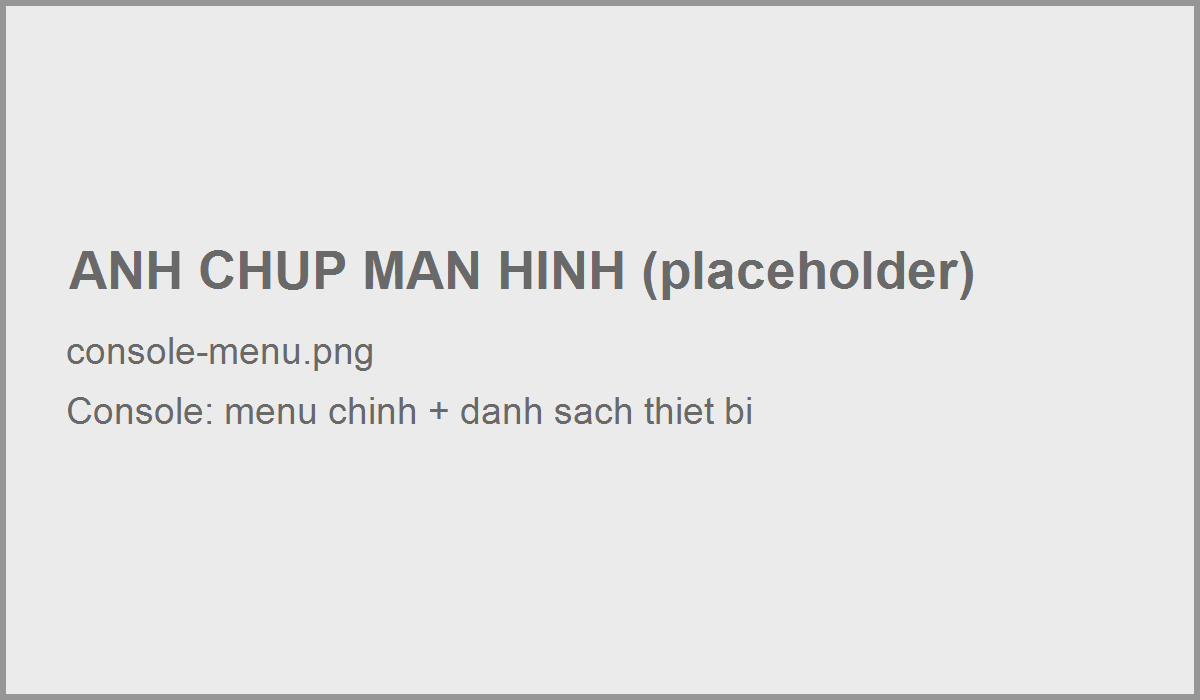
\includegraphics[width=0.92\textwidth]{figures/console-menu.png}
\caption{Console: menu chính và danh sách thiết bị}
\label{fig:console-menu}
\end{figure}

\begin{figure}[H]
\centering
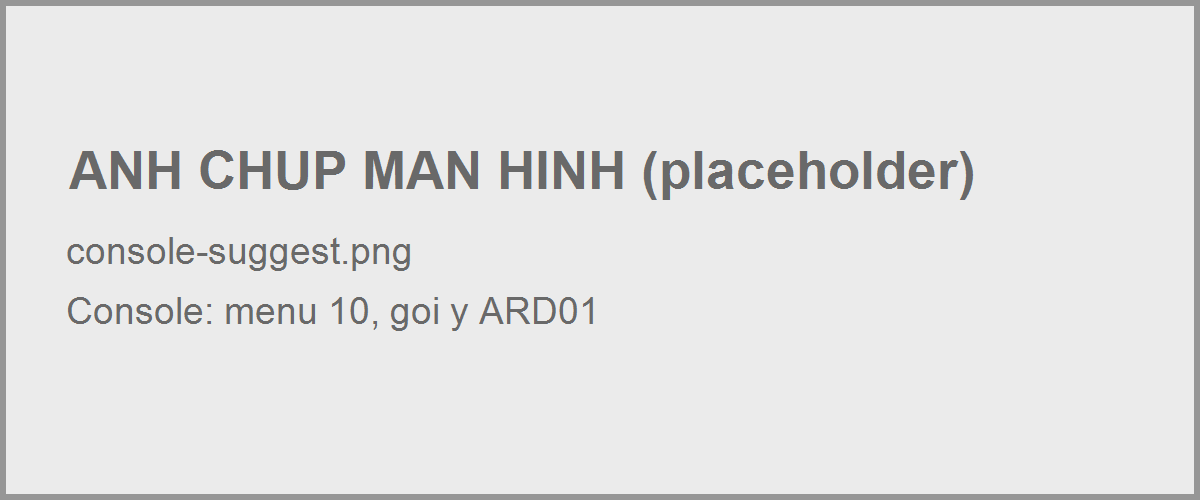
\includegraphics[width=0.92\textwidth]{figures/console-suggest.png}
\caption{Console: gợi ý thiết bị mượn kèm (menu 10)}
\label{fig:console-suggest}
\end{figure}

\section{Web}
\code{LabApp.exe} chạy máy chủ ở \code{127.0.0.1:8080}, phục vụ giao diện trong \code{web/} và API theo \code{docs/api.md}, rồi tự mở trình duyệt. Giao diện có bảy màn hình và một thanh đồng hồ giả lập có nút tua thời gian; mọi con số (quá hạn, gợi ý, vị trí hàng đợi) lấy từ API, không tính ở trình duyệt.

\subsection{Tổng quan}
Hiển thị tổng thiết bị, số đơn vị theo trạng thái, phiếu đang mở, phiếu quá hạn và phạt tạm tính, số người chờ/đang giữ, thiết bị mượn nhiều nhất.
\begin{figure}[H]
\centering
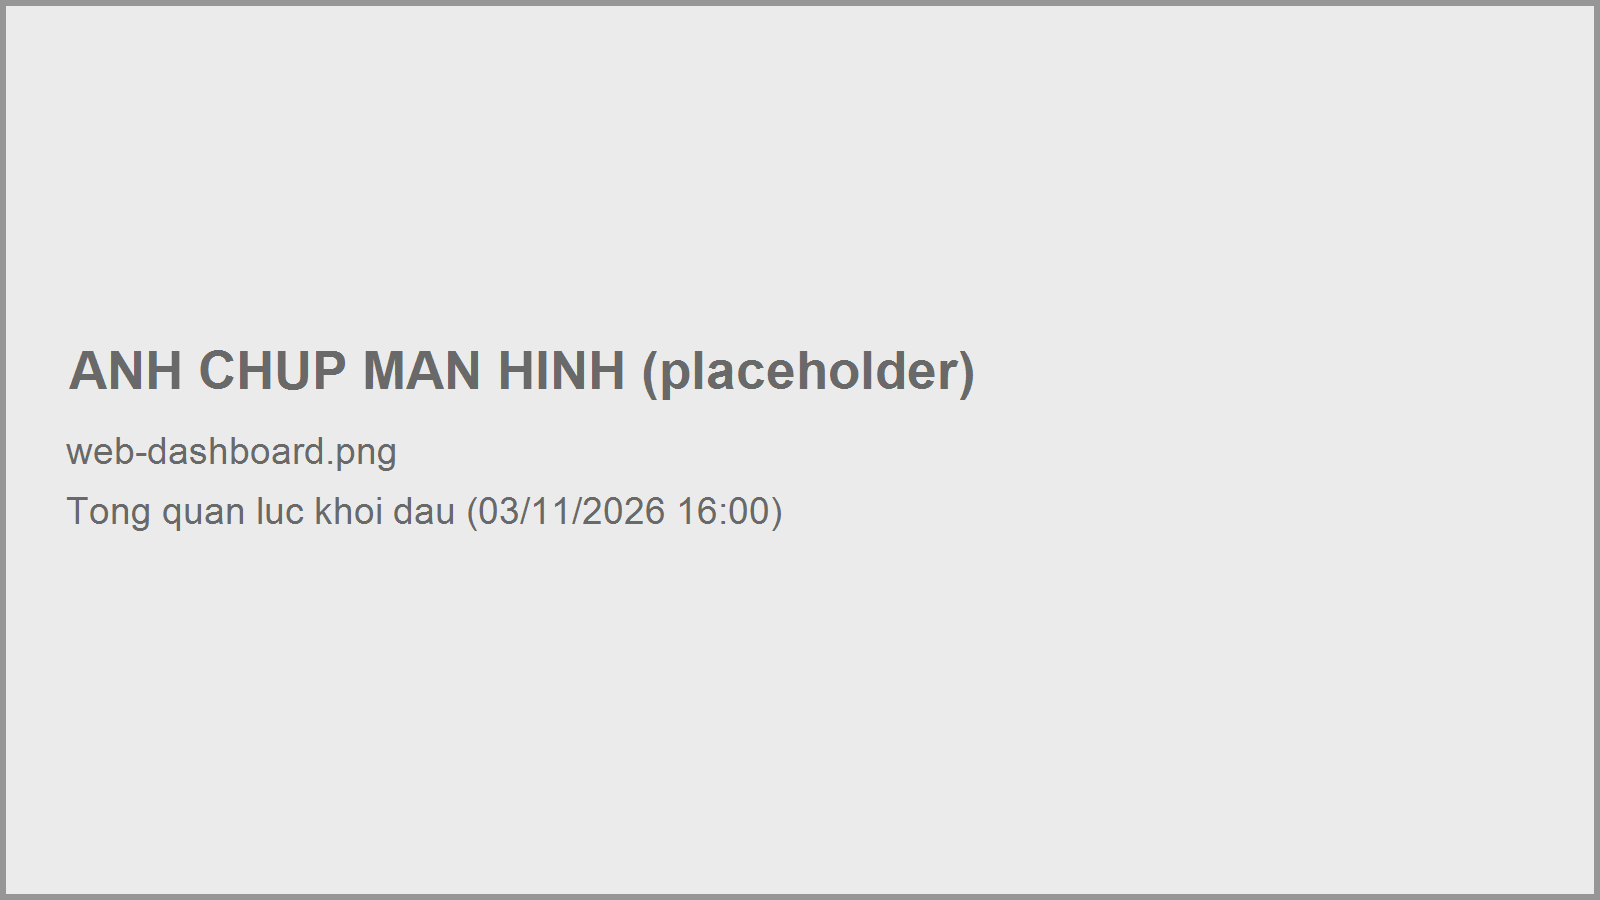
\includegraphics[width=0.95\textwidth]{figures/web-dashboard.png}
\caption{Màn Tổng quan ở trạng thái khởi đầu (03/11/2026 16:00)}
\label{fig:dashboard}
\end{figure}

\subsection{Thiết bị}
Danh sách thiết bị với thanh tỷ lệ \code{available/borrowed/onHold/maintenance} và trạng thái suy ra (M1); thêm, sửa, bảo trì, xoá.
\begin{figure}[H]
\centering
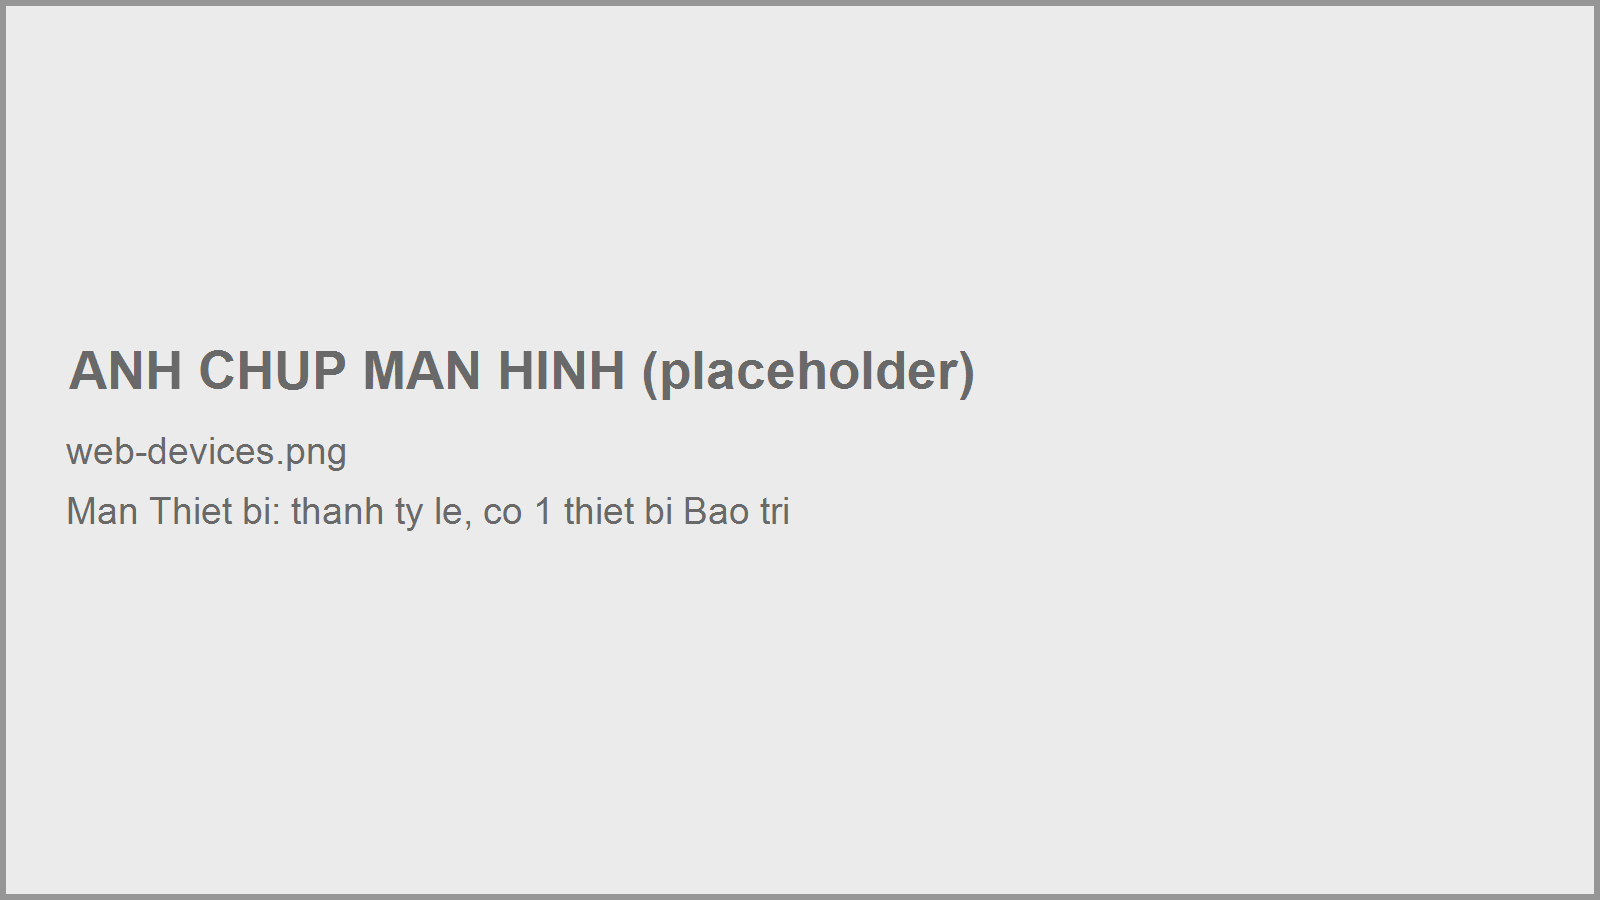
\includegraphics[width=0.95\textwidth]{figures/web-devices.png}
\caption{Màn Thiết bị: thanh tỷ lệ và trạng thái}
\label{fig:devices}
\end{figure}

\subsection{Mượn và gợi ý}
Chọn thiết bị vào giỏ; khung ``Thường được mượn kèm'' gợi ý theo cả giỏ (\code{suggestForBasket}) và tính lại mỗi khi thêm món.
\begin{figure}[H]
\centering
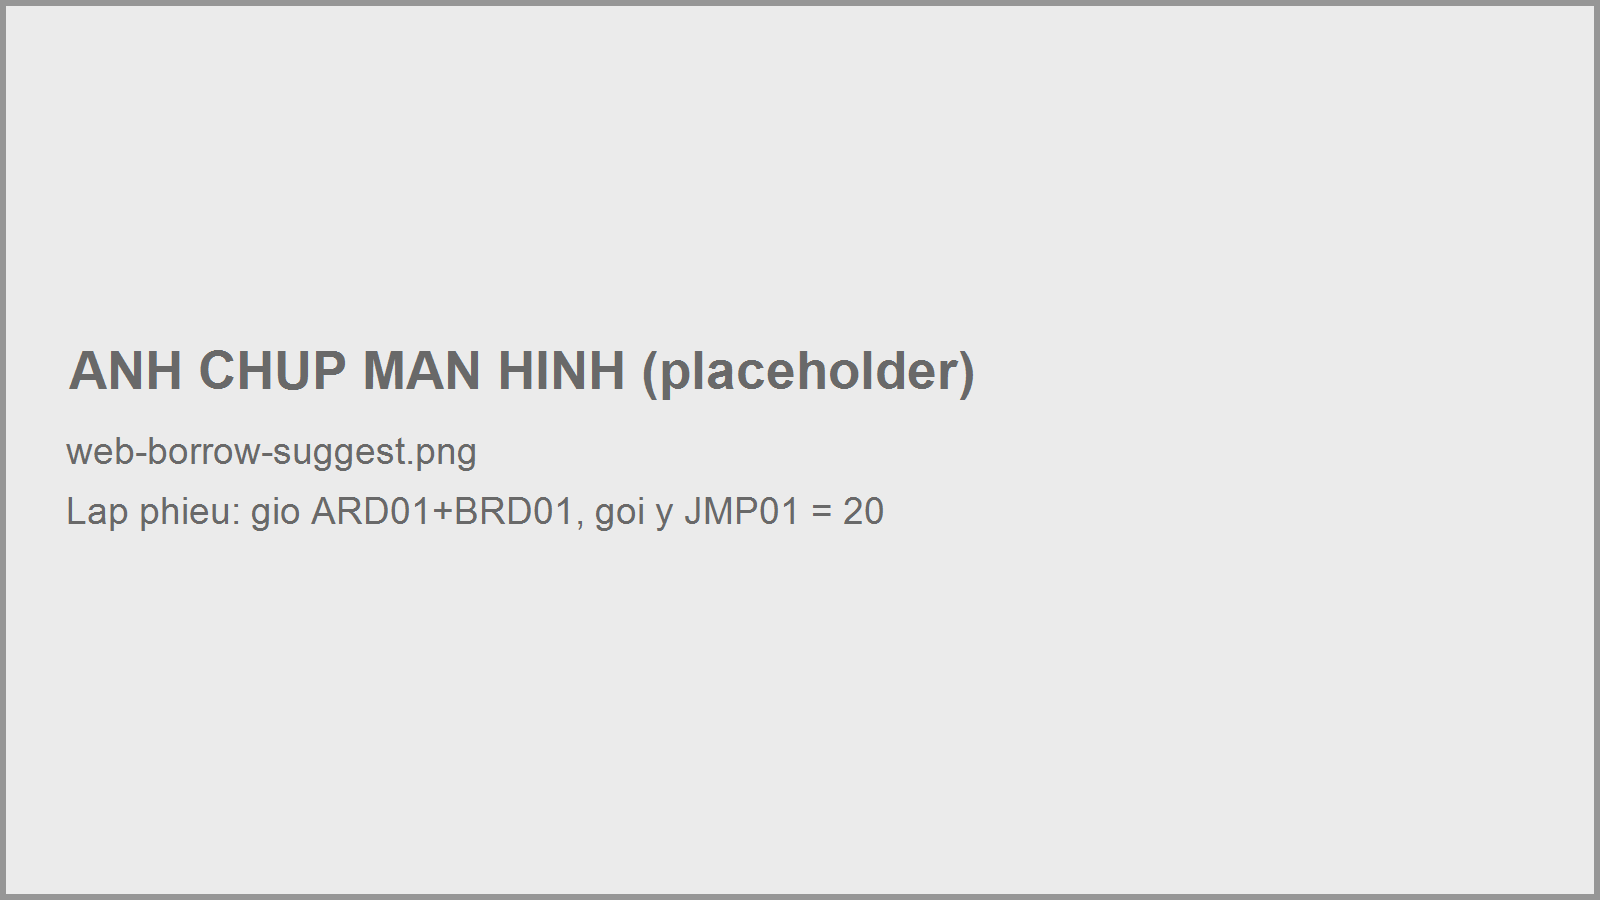
\includegraphics[width=0.95\textwidth]{figures/web-borrow-suggest.png}
\caption{Lập phiếu: giỏ ARD01 + BRD01, JMP01 đứng đầu với điểm cộng dồn 20}
\label{fig:borrow}
\end{figure}

\subsection{Trả thiết bị}
\begin{figure}[H]
\centering
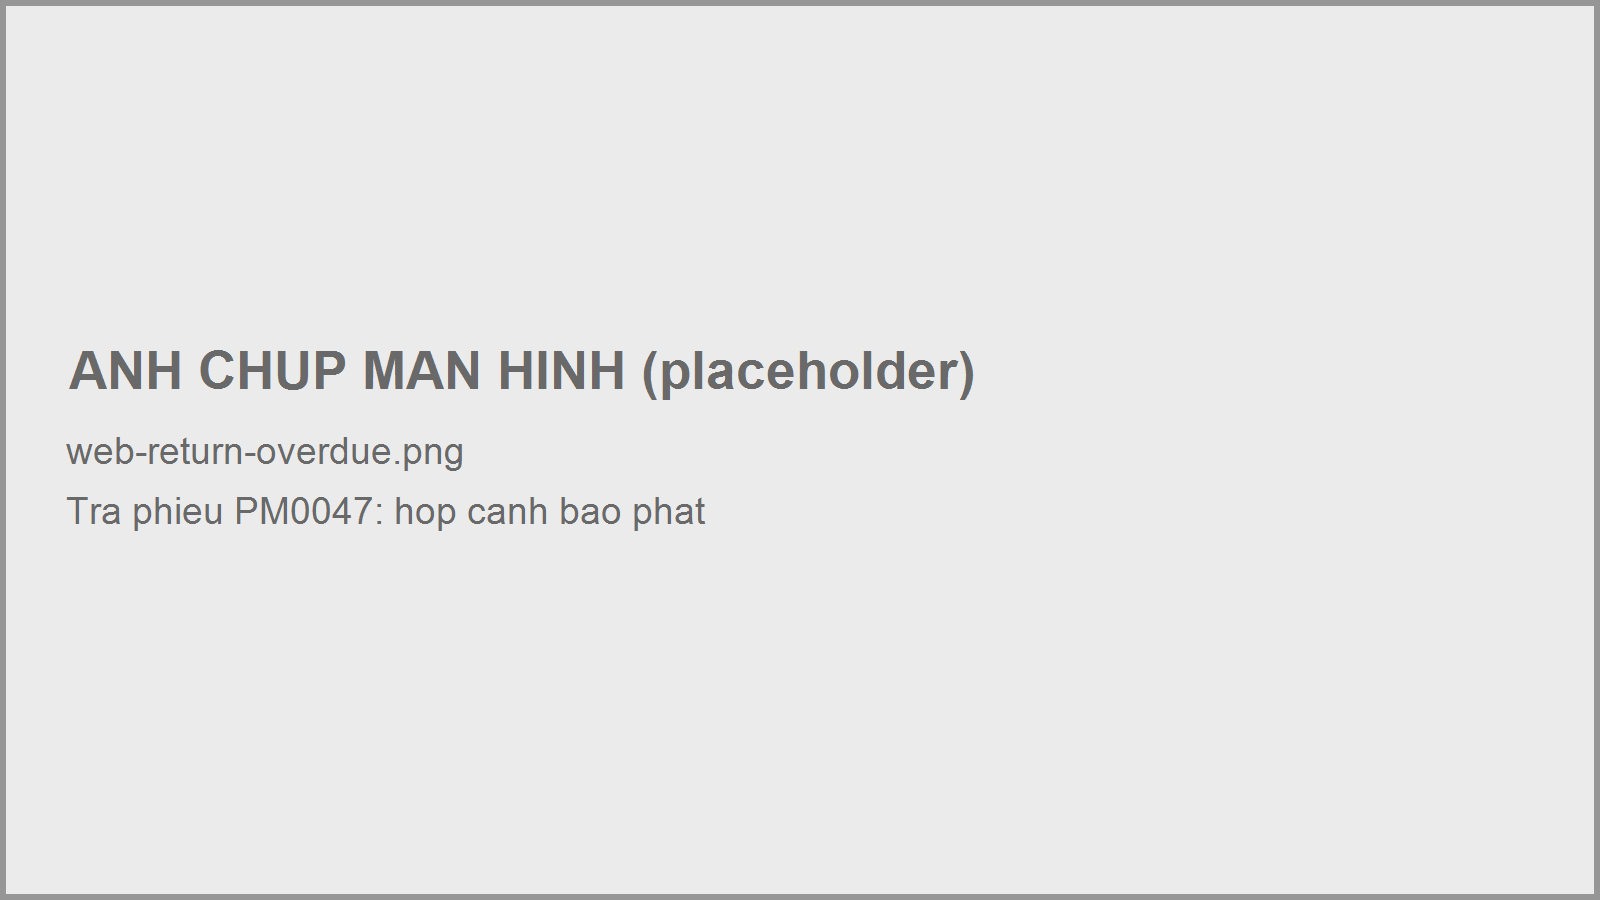
\includegraphics[width=0.95\textwidth]{figures/web-return-overdue.png}
\caption{Trả phiếu quá hạn: số ngày trễ và tiền phạt}
\label{fig:return}
\end{figure}

\subsection{Hàng đợi đặt trước}
Mỗi thiết bị một hàng: vị trí, trạng thái chờ/đang giữ, vòng đếm ngược 24 giờ, số lần lỡ hạn.
\begin{figure}[H]
\centering
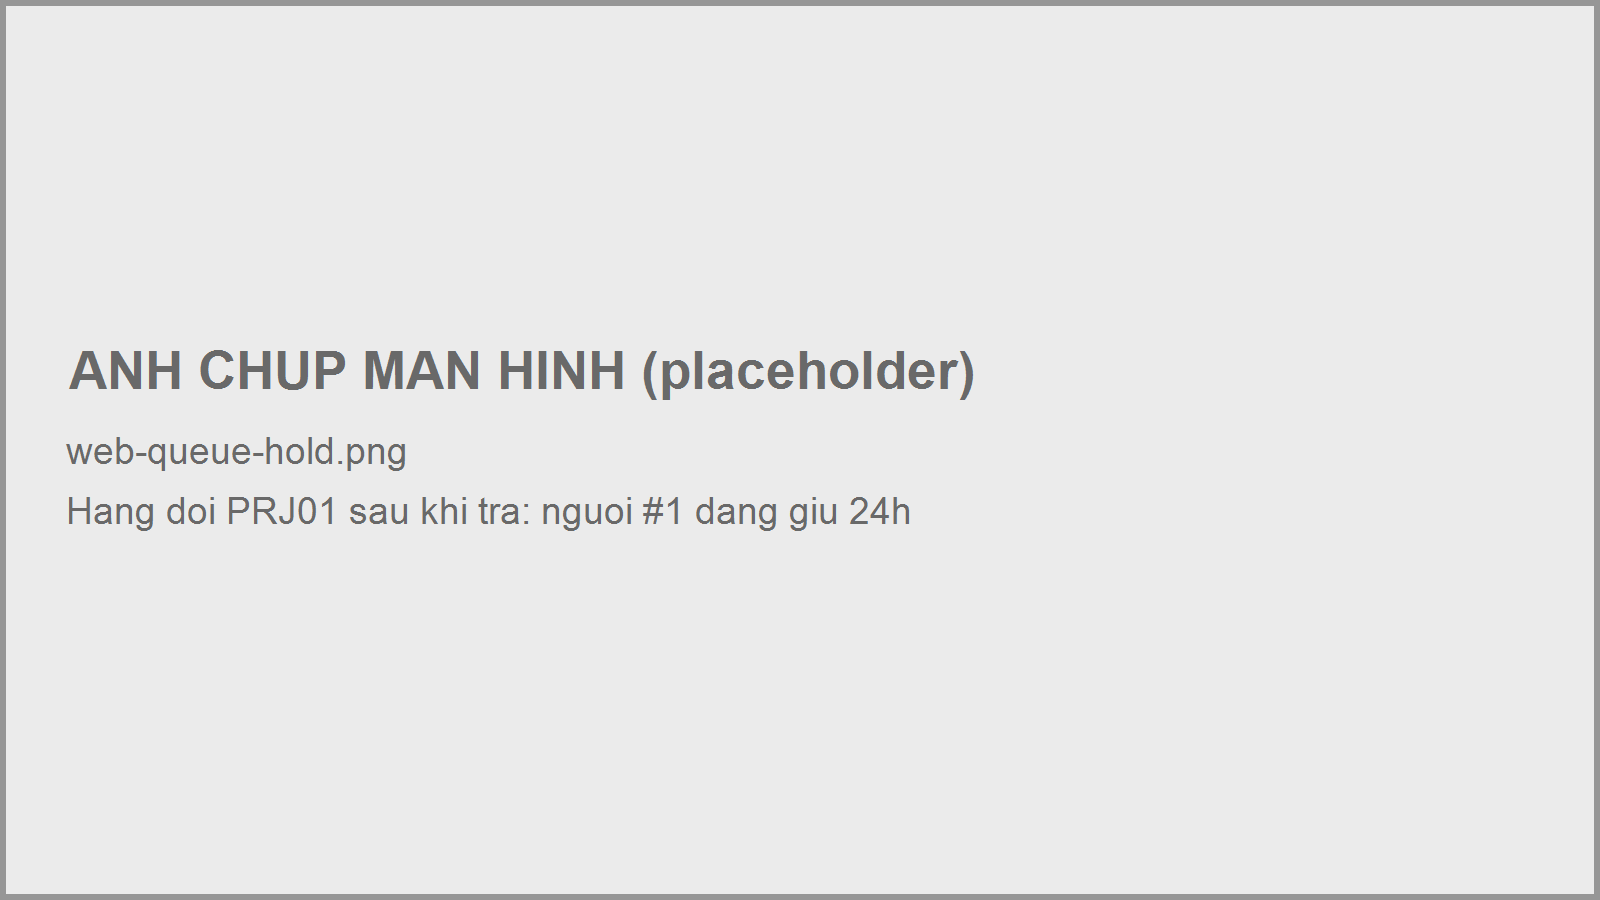
\includegraphics[width=0.95\textwidth]{figures/web-queue-hold.png}
\caption{Hàng đợi PRJ01 sau khi trả: người đứng đầu được giữ 24 giờ}
\label{fig:queue-hold}
\end{figure}
\begin{figure}[H]
\centering
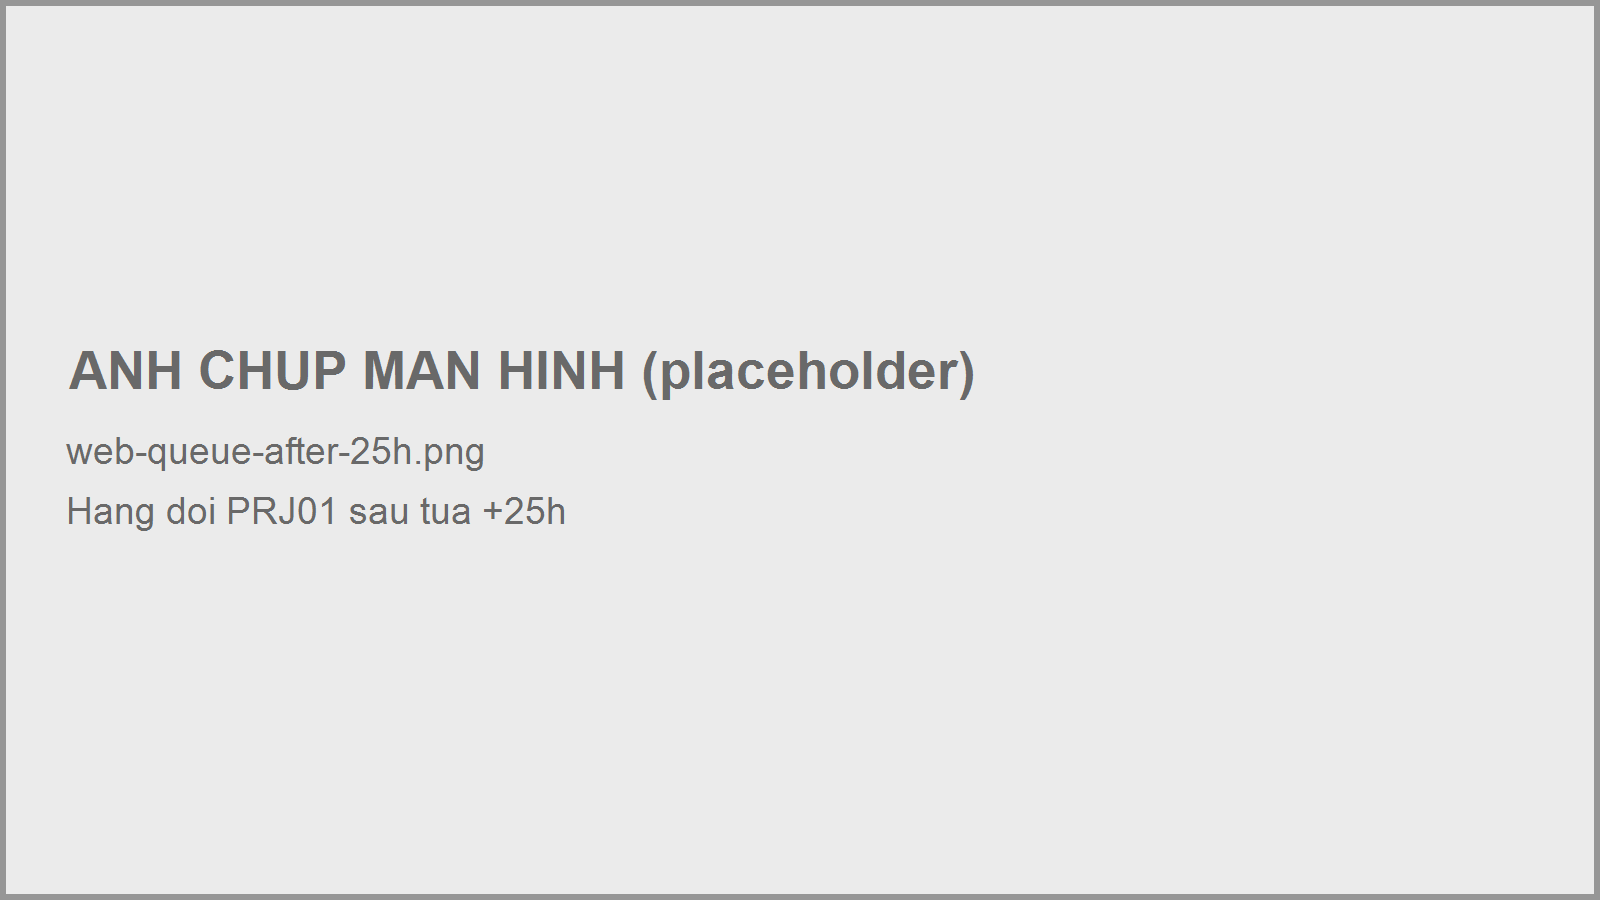
\includegraphics[width=0.95\textwidth]{figures/web-queue-after-25h.png}
\caption{Sau khi tua $+25$ giờ: người đầu lỡ hạn bị đẩy xuống cuối, người kế được giữ (hạn tính từ mốc cũ)}
\label{fig:queue-25h}
\end{figure}

\subsection{Quá hạn và lịch sử}
\begin{figure}[H]
\centering
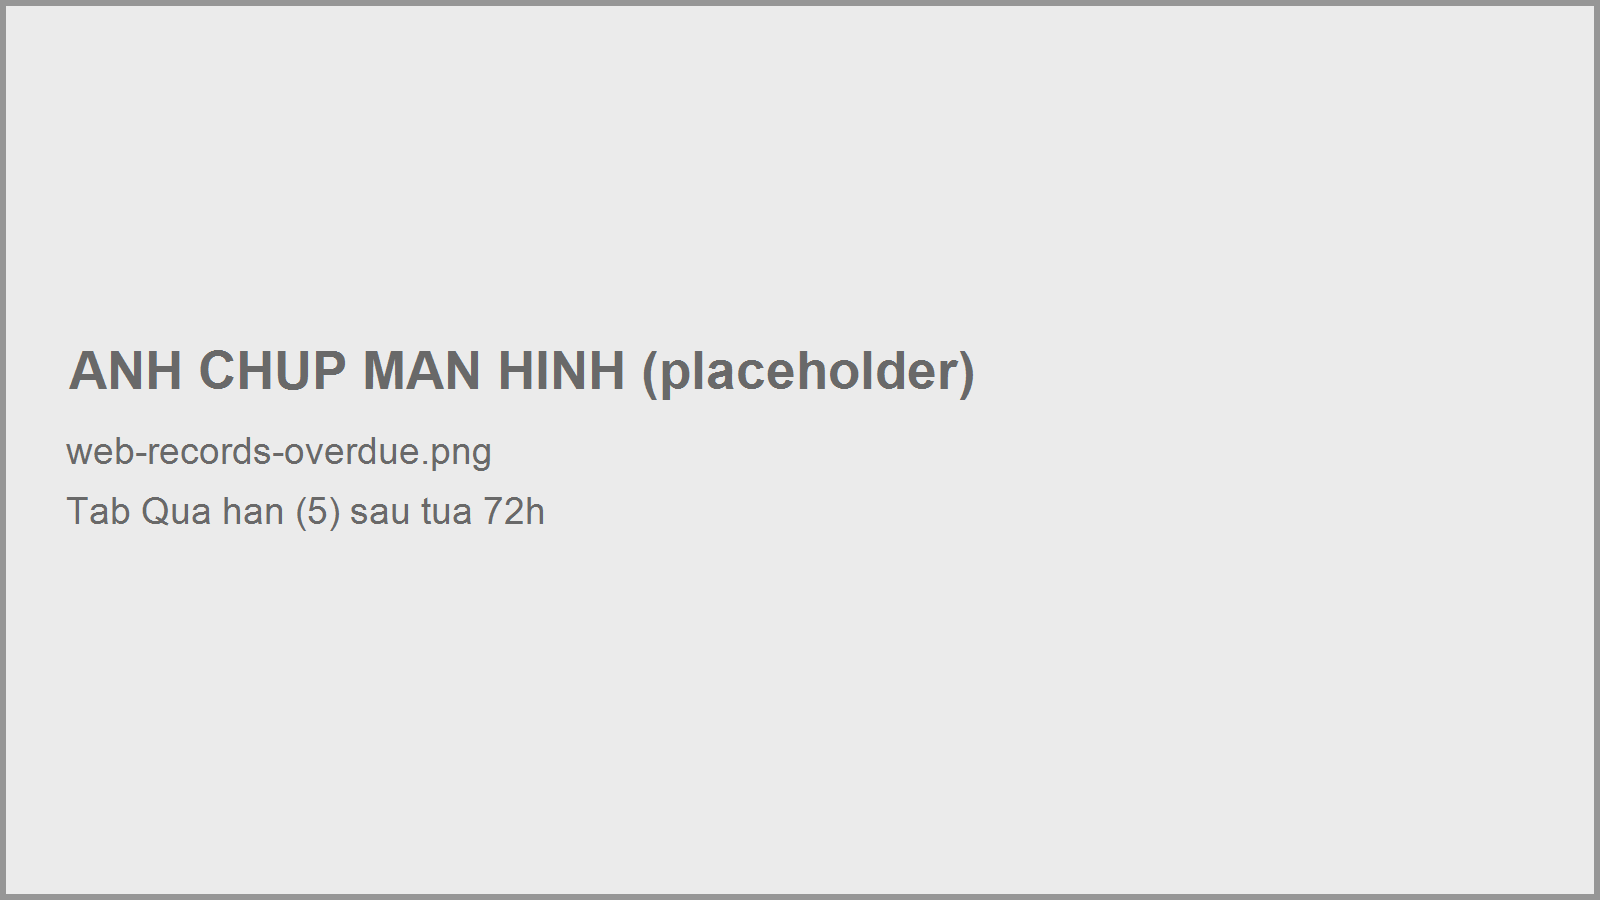
\includegraphics[width=0.95\textwidth]{figures/web-records-overdue.png}
\caption{Tab Quá hạn sau khi tua 72 giờ}
\label{fig:records}
\end{figure}

\subsection{Đồ thị mượn kèm}
Vẽ đồ thị với độ dày cạnh theo trọng số, lọc theo ngưỡng trọng số; chọn một đỉnh để xem top 3 mượn kèm.
\begin{figure}[H]
\centering
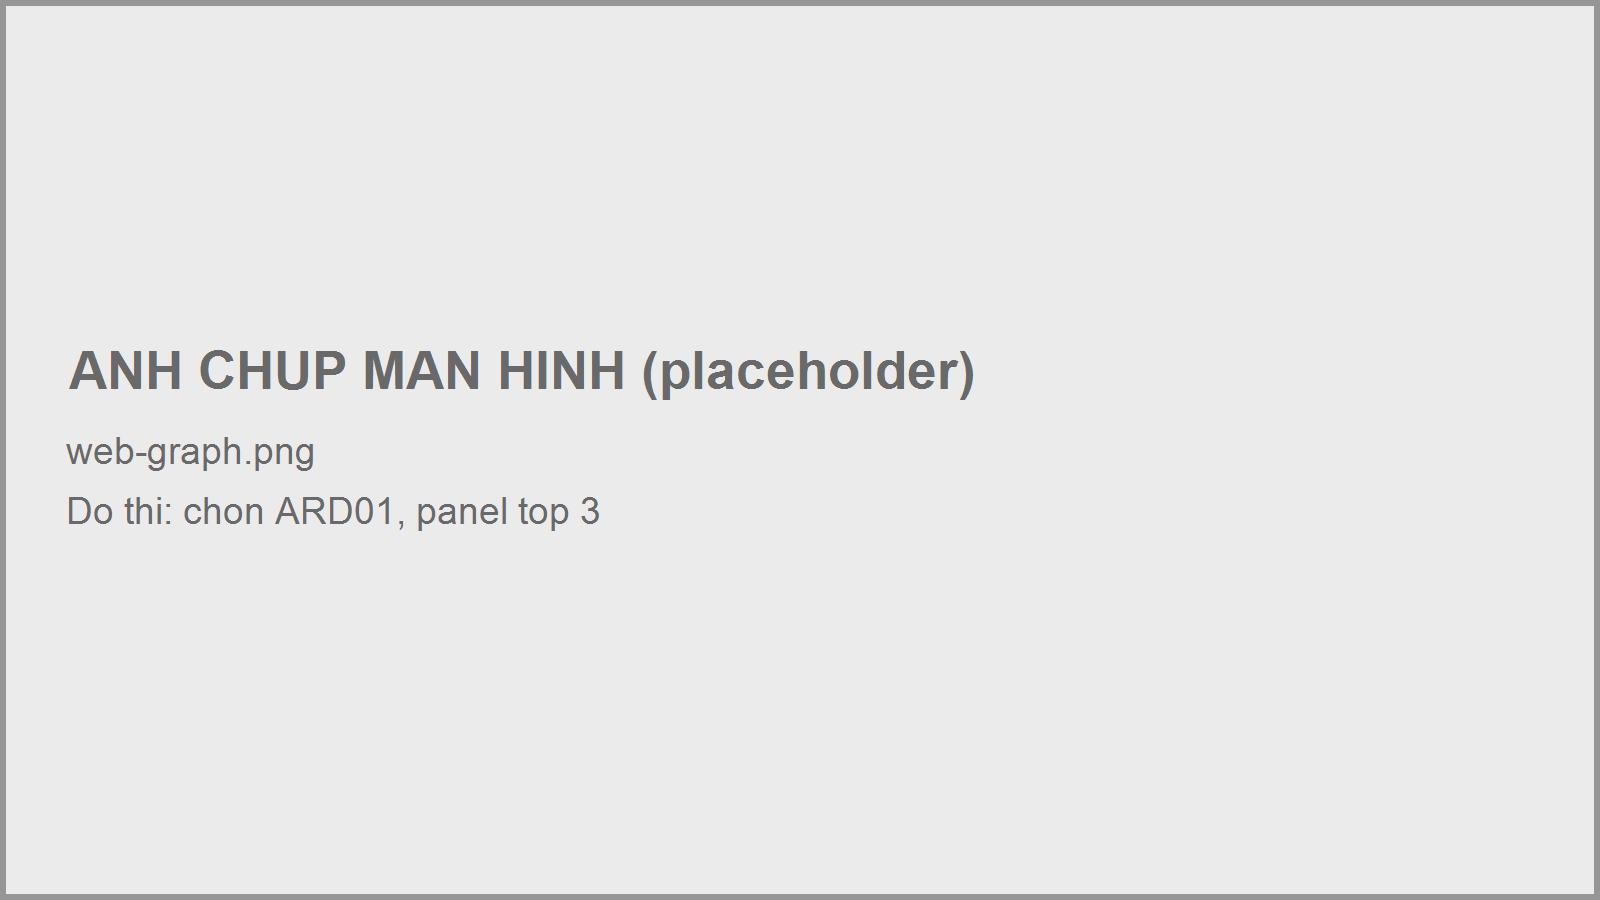
\includegraphics[width=0.95\textwidth]{figures/web-graph.png}
\caption{Màn đồ thị: chọn ARD01, panel top 3 thiết bị mượn kèm}
\label{fig:graph-ui}
\end{figure}

\chapter{Đánh giá, hạn chế và hướng phát triển}

\section{Đánh giá}
Đồ án đáp ứng đủ yêu cầu cơ bản và nâng cao của đề số 3:
\begin{itemize}
  \item ba cấu trúc dữ liệu (\code{DoublyLinkedList}, \code{LinkedQueue}, \code{Graph}) được tự cài đặt, không dùng container của STL trong lõi, có độ phức tạp ghi ngay trong mã và được kiểm thử (596 kiểm tra);
  \item hàng đợi đặt trước giữ 24 giờ, đẩy xuống cuối, loại sau hai lần lỡ, và chuyển quyền dây chuyền đúng khi tua nhiều giờ;
  \item đồ thị mượn kèm cho gợi ý top 3 theo thiết bị và theo cả giỏ;
  \item hai giao diện (console và web) dùng chung một lõi, cho số liệu giống nhau; dữ liệu lưu CSV và dựng lại phần suy ra khi nạp;
  \item bản phát hành chạy trên Windows 10 trở lên mà không cần cài thêm gì.
\end{itemize}
Điều rút ra: tách lõi khỏi giao diện ngay từ đầu giúp kiểm thử lõi độc lập, và việc chốt trước các quy ước nghiệp vụ (M1--M19) giúp mã, kiểm thử và báo cáo thống nhất.

\section{Hạn chế}
\begin{itemize}
  \item \textbf{Tra cứu theo mã là $O(n)$} (duyệt danh sách liên kết), và nhiều thao tác lặp lại phép tra này. Với vài chục thiết bị là không đáng kể, nhưng không mở rộng được cho hàng chục nghìn thiết bị.
  \item \textbf{Lưu CSV ghi lại toàn bộ tệp} sau mỗi thao tác, và \code{rename} sau \code{remove} không nguyên tử tuyệt đối: nếu mất điện đúng lúc đó, tệp \code{.tmp} còn nguyên dữ liệu mới nhưng phải khôi phục thủ công.
  \item \textbf{Một người dùng một tiến trình}: không đăng nhập, không phân quyền; không chạy đồng thời \code{app.exe} và \code{LabApp.exe} trên cùng thư mục dữ liệu.
  \item \textbf{Đồ thị chỉ ghi lịch sử}, không ``quên'': trọng số cũ vẫn ảnh hưởng gợi ý dù thói quen mượn đã đổi; phiếu 1 món (kể cả nhận từ hàng đợi) không đóng góp cạnh.
  \item \textbf{Đồng hồ giả lập} chỉ tiến, không lùi; thiếu \code{meta.csv} thì đồng hồ về 01/01/2026 00:00 (có cảnh báo).
  \item Mỗi thiết bị tối đa 1 đơn vị trong một phiếu (M7) và chưa có gia hạn phiếu.
\end{itemize}

\section{Hướng phát triển}
\begin{itemize}
  \item Thêm \textbf{bảng băm} hoặc \textbf{cây tìm kiếm cân bằng} để tra thiết bị theo mã trong $O(1)$ hoặc $O(\log n)$, giữ danh sách liên kết kép cho thứ tự hiển thị.
  \item Dùng \textbf{heap} để lấy top-$k$ trong $O(d + k\log d)$ và cho hàng đợi theo thời hạn (ưu tiên theo \code{holdUntil}).
  \item Cho đồ thị \textbf{trọng số suy giảm theo thời gian} để ưu tiên thói quen mượn gần đây.
  \item Hỗ trợ \textbf{nhiều phòng Lab}, gia hạn phiếu, nhắc hạn qua email, và lưu trữ bằng cơ sở dữ liệu nhẹ (SQLite) thay cho CSV.
  \item Bổ sung đăng nhập và phân quyền (thủ thư / sinh viên) nếu triển khai thực tế.
\end{itemize}

\section*{Phần có AI hỗ trợ}
\addcontentsline{toc}{section}{Phần có AI hỗ trợ}
Đồ án có dùng công cụ AI hỗ trợ lập trình, theo kế hoạch do sinh viên duyệt từng giai đoạn. \textbf{Claude Code} (Anthropic) hỗ trợ viết lõi cấu trúc dữ liệu, lưu CSV, console, máy chủ API, kiểm thử, tập lệnh đóng gói và bản nháp tài liệu; \textbf{Google Antigravity} (Gemini) hỗ trợ viết giao diện web theo đặc tả. Sinh viên chọn đề, chốt quy ước nghiệp vụ, duyệt kế hoạch và mã nguồn, chạy kiểm thử và chịu trách nhiệm giải thích cấu trúc dữ liệu cũng như độ phức tạp của sản phẩm nộp.


ocite{*}
\nocite{*}
\begin{thebibliography}{9}
\bibitem{clrs} T.~H. Cormen, C.~E. Leiserson, R.~L. Rivest, C.~Stein, \emph{Introduction to Algorithms}, 4th ed., MIT Press, 2022 (danh sách liên kết, hàng đợi, biểu diễn đồ thị bằng danh sách kề).
\bibitem{weiss} M.~A. Weiss, \emph{Data Structures and Algorithm Analysis in C++}, 4th ed., Pearson, 2013.
\bibitem{stroustrup} B.~Stroustrup, \emph{The C++ Programming Language}, 4th ed., Addison-Wesley, 2013.
\bibitem{cppref} \emph{cppreference.com}, tài liệu C++17. \url{https://en.cppreference.com}
\bibitem{httplib} Y.~Yhirose, \emph{cpp-httplib}, thư viện HTTP header-only cho C++. \url{https://github.com/yhirose/cpp-httplib}
\bibitem{json} N.~Lohmann, \emph{JSON for Modern C++}. \url{https://github.com/nlohmann/json}
\bibitem{de} Trần Tuấn Kiệt, \emph{Đề đồ án số 3 --- Quản lý mượn trả thiết bị và gợi ý đồ dùng thực hành}, môn Thực hành Cấu trúc dữ liệu và Giải thuật, HCMUS.
\end{thebibliography}


\end{document}
